% This file makes a web version of the blueprint
% It should include all the \usepackage needed for this version.
% The template includes standard AMS packages.
% It is otherwise a very minimal preamble (you should probably at least
% add cleveref and tikz-cd).

\documentclass{report}

\usepackage{amssymb, amsthm, amsmath}
\usepackage{hyperref}
\usepackage[showmore, dep_graph, web, thms=theorem+proposition+lemma+corollary+definition+tactic]{blueprint}

% In this file you should put all LaTeX macros and settings to be used both by
% the pdf version and the web version.
% This should be most of your macros.

% The theorem-like environments defined below are those that appear by default
% in the dependency graph. See the README of leanblueprint if you need help to
% customize this. 
% The configuration below use the theorem counter for all those environments
% (this is what the [theorem] arguments mean) and never resets it.
% If you want for instance to number them within chapters then you can add
% [chapter] at the end of the next line.
\newtheorem{theorem}{Theorem}
\newtheorem{proposition}[theorem]{Proposition}
\newtheorem{lemma}[theorem]{Lemma}
\newtheorem{corollary}[theorem]{Corollary}

\theoremstyle{definition}
\newtheorem{definition}[theorem]{Definition}
% This file makes a web version of the blueprint
% It should include all the \usepackage needed for this version.
% The template includes standard AMS packages.
% It is otherwise a very minimal preamble (you should probably at least
% add cleveref and tikz-cd).

\documentclass{report}

\usepackage{amssymb, amsthm, amsmath}
\usepackage{hyperref}
\usepackage[showmore, dep_graph]{blueprint}


% In this file you should put all LaTeX macros and settings to be used both by
% the pdf version and the web version.
% This should be most of your macros.

% The theorem-like environments defined below are those that appear by default
% in the dependency graph. See the README of leanblueprint if you need help to
% customize this. 
% The configuration below use the theorem counter for all those environments
% (this is what the [theorem] arguments mean) and never resets it.
% If you want for instance to number them within chapters then you can add
% [chapter] at the end of the next line.
\newtheorem{theorem}{Theorem}
\newtheorem{proposition}[theorem]{Proposition}
\newtheorem{lemma}[theorem]{Lemma}
\newtheorem{corollary}[theorem]{Corollary}

\theoremstyle{definition}
\newtheorem{definition}[theorem]{Definition}
% This file makes a web version of the blueprint
% It should include all the \usepackage needed for this version.
% The template includes standard AMS packages.
% It is otherwise a very minimal preamble (you should probably at least
% add cleveref and tikz-cd).

\documentclass{report}

\usepackage{amssymb, amsthm, amsmath}
\usepackage{hyperref}
\usepackage[showmore, dep_graph]{blueprint}


% In this file you should put all LaTeX macros and settings to be used both by
% the pdf version and the web version.
% This should be most of your macros.

% The theorem-like environments defined below are those that appear by default
% in the dependency graph. See the README of leanblueprint if you need help to
% customize this. 
% The configuration below use the theorem counter for all those environments
% (this is what the [theorem] arguments mean) and never resets it.
% If you want for instance to number them within chapters then you can add
% [chapter] at the end of the next line.
\newtheorem{theorem}{Theorem}
\newtheorem{proposition}[theorem]{Proposition}
\newtheorem{lemma}[theorem]{Lemma}
\newtheorem{corollary}[theorem]{Corollary}

\theoremstyle{definition}
\newtheorem{definition}[theorem]{Definition}
% This file makes a web version of the blueprint
% It should include all the \usepackage needed for this version.
% The template includes standard AMS packages.
% It is otherwise a very minimal preamble (you should probably at least
% add cleveref and tikz-cd).

\documentclass{report}

\usepackage{amssymb, amsthm, amsmath}
\usepackage{hyperref}
\usepackage[showmore, dep_graph]{blueprint}


\input{macros/common}
\input{macros/web}

%\home{https://LiamSchilling.github.io/AutomatePolynomial}
%\github{https://github.com/LiamSchilling/AutomatePolynomial}
%\dochome{https://LiamSchilling.github.io/AutomatePolynomial/docs}

\title{AutomatePolynomial}
\author{Liam Schilling}

\begin{document}
\maketitle
\input{content}
\end{document}

%\home{https://LiamSchilling.github.io/AutomatePolynomial}
%\github{https://github.com/LiamSchilling/AutomatePolynomial}
%\dochome{https://LiamSchilling.github.io/AutomatePolynomial/docs}

\title{AutomatePolynomial}
\author{Liam Schilling}

\begin{document}
\maketitle
% In this file you should put the actual content of the blueprint.
% It will be used both by the web and the print version.
% It should *not* include the \begin{document}
%
% If you want to split the blueprint content into several files then
% the current file can be a simple sequence of \input. Otherwise It
% can start with a \section or \chapter for instance.

\seca{Introduction}
\label{sec:intro}

\secb{Organization of the Blueprint}

The blueprint is organized as follows: The rest of Section~\ref{sec:intro} examines previous work in proof automation and polynomials in Lean, and provides a brief comparison with the approach taken in our work. Section~\ref{sec:reflection} describes our approach to proof by reflection and outlines a model for its implementation. This section will also be of interest to readers curious about our use of type-class inference in proof automation. Section~\ref{sec:univariate} details the implementation of each part of the model for univariate polynomials. Readers interested in using the univariate system for proof automation should be directed specifially to Section~\ref{sec:tactics}. Section~\ref{sec:multivariate} addresses ongoing work towards a system for multivariate polynomials.

\secb{Automation in Lean}
\label{sec:automation}

Previous work outlines a number of approaches to proof automation in Lean 4, each with different advantages and preferred applications. The Ring of Integers project \cite{RingOfIntegers2025} covers proof automation methods in Lean extensively and may be referenced for a more technical address of the topic. This blueprint will introduce and evaluate proof automation strategies in previous work as it relates to our approach. We broadly refer to these strategies as \emph{proof by reflection}.

One proof-by-reflection paradigm is white-box automation \cite{Aesop2023}, in which the automation procedure is transparent and simple enough for users to trace and predict how an application will deal with their goals. Although these solutions tend to be narrow-application in terms of the goals they can deal with, they are highly extensible to different contexts since the user can understand and customize them. Search tactics such as \tacticinline{aesop} \cite{Aesop2023} and reflection models such as LeanSSR \cite{SmallScaleReflection2024} are common examples of such automation. While alternative proof-by-reflection paradigms such as LLMs are more general-application, they tend to be more brittle to changes in context and difficult to debug due to their complexity. There have even been recent efforts to make these solutions more usable by integrating them as assistants in the interactive-proving process, using them to resolve subgoals instead of relying on them for complex theorems. Lean Copilot \cite{LeanCopilot2025}, for instance, integrates their LLM implementation with aesop’s search, resulting in a white-box solution with some of the general-application benefits of LLM automation.

Popular implementations also tend to be native to Lean since they are easier to use, entail less dependencies, and enjoy the benefits of Lean's powerful tactics and metaprogramming. For instance, Lean Copilot \cite{LeanCopilot2025} implements their Lean declarations in C++, to which Lean compiles directly. Moreover, LeanSSR \cite{SmallScaleReflection2024} emphasizes how Lean is a great candidate for implementation of their reflection model because of its powerful metaprogramming support. LeanSSR also discusses how Lean's flexible tactics for goal manipulation result in convenient ``last-mile automation'' strategies, where the user only needs to manipulate the goal to a point where it can be automatically resolved by some form of reduction. For example, the built-in tactics \tacticinline{rfl} and \tacticinline{simp} automate a variety of goals by reducing them according to simple rules. Our native approach makes generous use of these last-mile automation strategies. Overall, it seems that native, white-box automation is a leading contender for Lean.

Type-class inference, which our project employs to construct computable representations, seems unexplored as a search method compared to metaprogramming and search tactics. We find in our project that it greatly simplifies resolving goals that can be split into similar subgoals without much additional verification at each step. However, it requires additional help from tactics when verification beyond the scope of the procedure is necessary at any step (see Section~\ref{sec:sensitive}).

\secb{Polynomials in Lean}

Previous work with polynomials in Lean highlights how a lack of computable representations can limit the impact of a formalization. As described by Wieser \cite{ComputationalPolynomialsFinsupps}, polynomials in Mathlib are non-computable because they are implemented using the \leaninline{Finsupp} type for finitely supported functions, whose underlying support set may not have decidable membership. An early Lean 3 formalization \cite{MasonStothers2018} aimed to prove the Mason Stothers Theorem. The project achieved this goals, though it first had to build up the necessary background in number theory and polynomials. A later project \cite{MasonStothers2024} which achieved the same formalization using Lean 4’s Mathlib noted that the previous project’s rejection of established machinery limited its application and reusability. This is because its results cannot be easily related to the standard Mathlib definitions used in other projects.

Some projects take advantage of the computational benefits of machine formalization, implementing algorithms on polynomials in Lean. One project implemented Buchberger’s Algorithm \cite{Buchbergers2019} but noted that Mathlib’s non-computable polynomial representation made it ineffective for their application. The authors implemented their own polynomials for use in their implementation, limiting its reusability similarly to the projects dealing with the Mason Stothers Theorem. Another project \cite{UnivariateSolutions2022} implemented algorithms for finding solutions to univariate polynomials, but built their mathematical machinery---all the way from natural numbers---from scratch. Although an impressive look into what it takes to formalize such mathematical background, this definitional separation limits the project in the same ways as the previous one.

Recent work focuses on more computable representations and automations for polynomials in Lean. Davenport \cite{ComputationalPolynomials2024} outlines the design decisions towards implementing such a representation and some operations on it. However, he does not detail any proof of correctness for those operations, and instead discusses verification using SageMath. Another approach to automation is Wieser’s \tacticinline{polyrith} tactic \cite{Polyrith}, which uses SageMath to compute necessary parameters for resolving a goal with Mathlib’s \tacticinline{linear\_combination} tactic. It is a highly effective white-box method for polynomials over fields. In both these methods, proof automation is non-native. Our approach introduces a computable representation and correctness-verified operations all native to Lean. Furthermore, the representations do not require polynomials defined over fields, only commutative semirings in the most specific cases, making the solution more general than polyrith in this aspect.

The Ring of Integers project \cite{RingOfIntegers2025} briefly discusses construction of computable representations based on expressions in the current goal as a proof automation method. They also discuss their list-based implementation of a computable representation for polynomials which is similar to our list-based implementation. However, they explain as a limitation that their implementation does not provide such a way to automatically construct this representation. This type of automated construction is central to our approach and is achieved using the unexplored method of type-class inference (recall Section~\ref{sec:automation}). For these reasons, we consider this aspect the most novel contribution of our work.

It should be noted that the powerful \tacticinline{grind} tactic \cite{Grind} for automated reasoning over finite algebras became available in Lean during work on this project. For its Gröbner basis computations, the system ships with a computable representation of polynomials implemented by the \leaninline{Poly} type (see \href{https://github.com/leanprover/lean4/blob/master/src/Init/Grind/Ring/Poly.lean}{\texttt{Poly.lean}}) and automated construction methods for it. It is still unclear how those automated construction methods compare to those used in our project, though future work may explore this question as well as how adoption of the convenient \leaninline{Poly} type could improve our system.

\seca{Reflection by Inference}
\label{sec:reflection}

\secb{Representation Inference}

Lean's type-class inference is a powerful tool for automatically constructing instances of a parameterized type. Our approach to proof-by-reflection, which we will call \emph{reflection by inference}, employs type-class inference to construct computable representations of target properties. First, we will briefly discuss type-class inference. Instance declarations are the blueprint for this process; each declaration states the parameter of the type it instantiates, admits any type class instances it requires as input, and specifies how to construct the target instance from these inputs. As displayed in Figure~\ref{fig:inference}, type-class inference is a depth-first search which, at each step, checks all instance declarations that match the current goal. For more details on type-class inference, consult the \textit{Theorem Proving in Lean 4} handbook \cite{TypeClasses}.

Lean's type-class inference is central to our reflection model and we will refer to it as the \emph{inference procedure}. In our case, the types we will construct are of computable representations of the target properties parameterized over polynomials. We will refer to these computable representions as \emph{representations} and the type classes that contain instances of them as \emph{reflection classes}. As addressed in Figure~\ref{fig:model}, reflection classes are generic to the representations they contain. It follows that the inference procedure is generic to computable representations of the target properties. We will refer to instance declarations for reflection classes as \emph{inference rules}. Once the reflection classes and inference rules are declared, we may implement \emph{tactics} that perform the inference procedure to resolve goals. These tactics rewrite the target property as the constructed computable representation so that the goal can be resolved by last-mile automation tactics. Recall that the LeanSSR project \cite{SmallScaleReflection2024} discusses last-mile automation.

\secb{Reflection Model}

The reflection-by-inference model in Figure~\ref{fig:model} guides our implementation of the system for polynomials. We ensure levels of modularity with respect to the target property and the representation of that property by specifying three levels of abstraction: The \emph{signature} declares inference rules for generic reflection classes. The \emph{interface} extends multiple signatures with a specified reflection class that asserts the target property. At this level, tactics may be implemented for generic representations. The \emph{implementation} instantiates an interface with a specified representation of the target property and implements the rules declared in the signatures.

\begin{figure}
\centering
\caption{Visualization of the reflection-by-inference model.}
\label{fig:model}
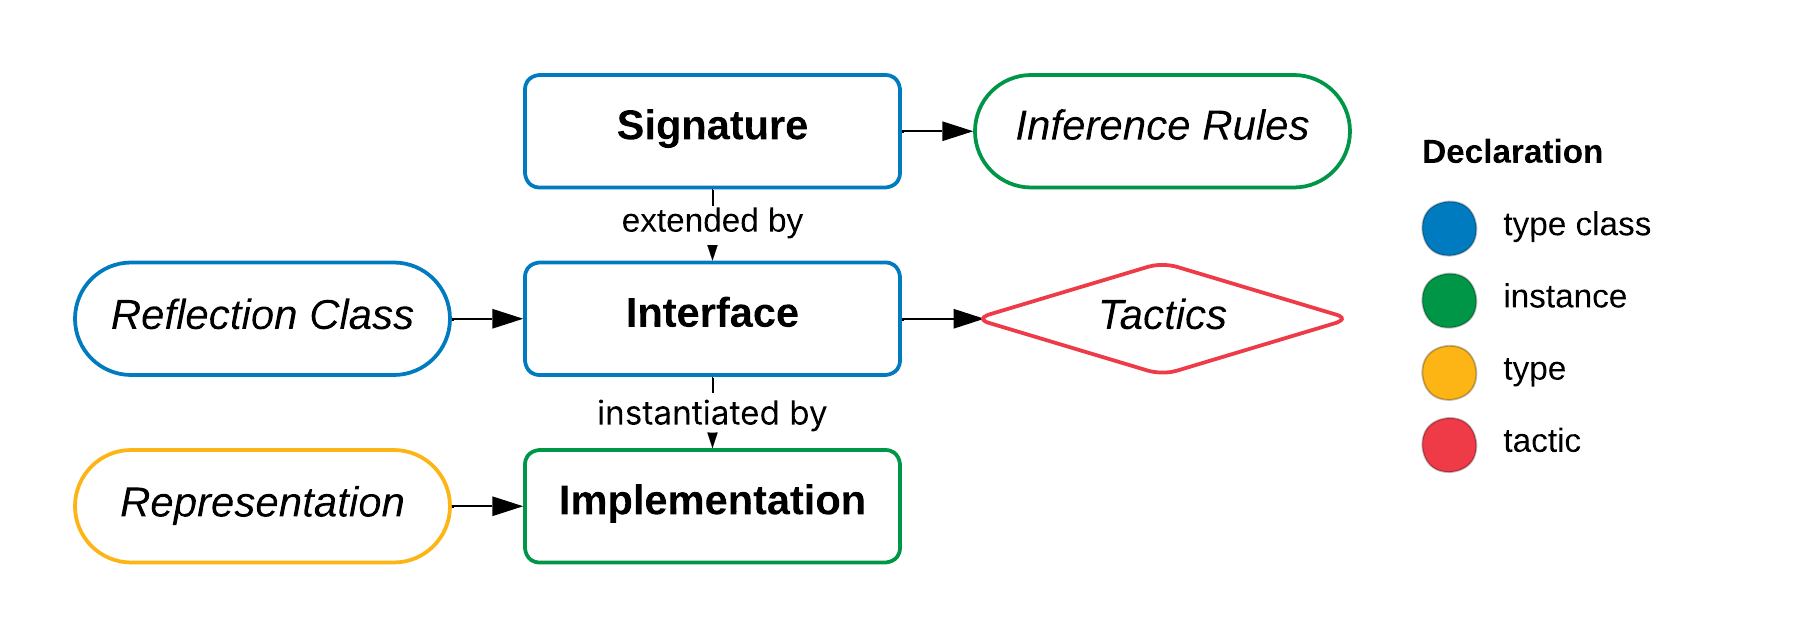
\includegraphics[width=5in]{architecture.png}
\end{figure}

\begin{figure}
\centering
\caption{The inference procedure constructs an upper bound on the degree of a polynomial.}
\label{fig:inference}
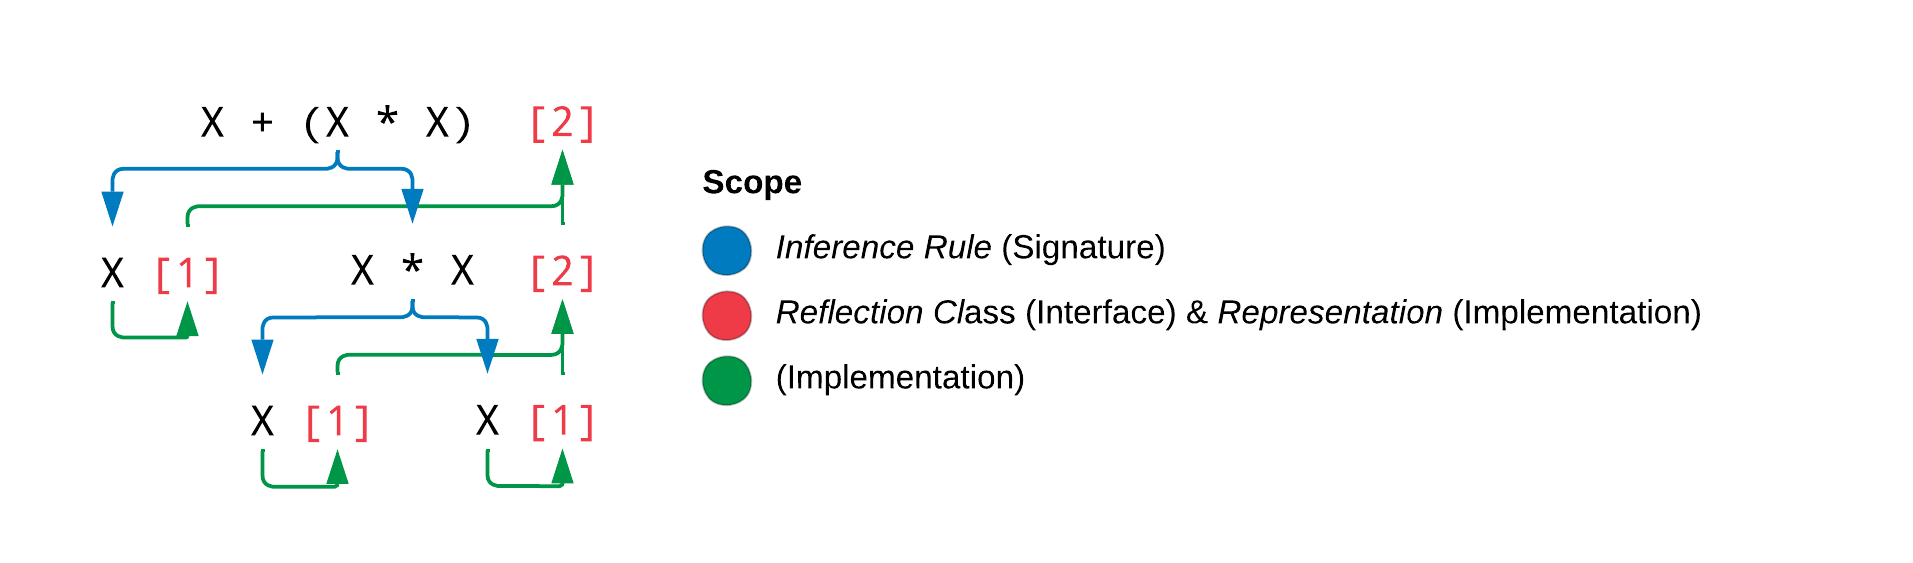
\includegraphics[width=6in]{inference.png}
\end{figure}

\secb{Sensitive Inference Procedure}
\label{sec:sensitive}

Although the inference procedure is effective for target properties with inference rules that require only the simple input instances without extra conditions, it is limited for properties that require extra assumptions at each step. For example, inference for exact degrees and leading coefficients requires that leading terms do not cancel at each \leaninline{+}, \leaninline{*}, or \leaninline{\^{}} step. To address this issue, we implement the \emph{sensitive inference procedure} which is invoked by Tactic~\ref{tac:infer_instance_trying}.

\begin{tactic}[\tacticinline{infer\_instance\_trying}]
\label{tac:infer_instance_trying}
\lean{Lean.MVarId.synthInstanceTrying, «tacticInfer_instance_trying<:>_»}
\leanok
Performs a depth-first search which, at each step, applies a provided helper tactic \tacticinline{t} then checks all instance declarations that match the current goal. Unlike Lean's type-class inference, this procedure supports instance declarations that require assumptions that cannot be resolved by type-class instances, handling them with the helper tactic instead. The syntax is \tacticinline{infer\_instance\_trying}\leaninline{ <:> }\tacticinline{t}.
\begin{lstlisting}
open Nat

class IsDouble (n : ℕ) where
  m : ℕ
  h : n = 2 * m

instance (h : n % 2 = 0) : IsDouble n :=
  ⟨n / 2, (Nat.mul_div_cancel' (dvd_of_mod_eq_zero h)).symm⟩

example : IsDouble 4 := by infer_instance_trying <:> decide
\end{lstlisting}
\end{tactic}

\seca{Univariate System}
\label{sec:univariate}

\secb{Inference Rules}

We define type classes that declare groups of inference rules. These classes may be extended to construct specifications for inference procedures requiring assumptions of varying strenghts (e.g. from nonsensitive to very sensitive). An implementation of an inference procudure must meet its specificaitions by implementing its inference rules.

Because we differentiate between inference rules for bases cases and inference rules for recursive cases of polynomials, inference procedures may be sensitive to varying degrees. To demonstrate:

\begin{itemize}
\item \textbf{Nonsensitive}: greedy degree upper bound inference is nonsensitive as it never requires additional assumptions beyond the input instances
\item \textbf{Somewhat sensitive}: leading coefficient inference is sensitive in recursive cases but nonsensitive in base cases
\item \textbf{Very sensitive}: exact degree inference is sensitive as it always requires additional assumptions beyond the input instances
\end{itemize}

It should also be emphasized that when we assert that we require some type in the following definitions, we mean that we must be provided a way to compute a member of that type, not just that such a member exists, given the current assumptions as input.

\begin{definition}[Nonsensitive rules for base cases]
\label{def:BaseReflection}
\lean{Polynomial.Rfl.BaseReflection}
\leanok
Given a semiring $R$ and a property of polynomials $T:R[x] \to \mathtt{Type}$, nonsensitive inference of $T$ for base cases of $R[x]$ requires that we have the following.
\begin{itemize}
\item $T(0)$
\item $T(c)$ for $c \in R$
\item $T(x)$
\item $T(x ^ n)$ for $n \in \mathbb{N}$
\end{itemize}
The $T(x ^ n)$ case is not strictly necessary here and could have been analyzed as a result of recursive cases. However, $T(x ^ n)$ often has a nice closed form so it is included here for efficiency.
\end{definition}

\begin{definition}[Nonsensitive rules for recursive cases]
\label{def:ClosureReflection}
\lean{Polynomial.Rfl.ClosureReflection}
\leanok
Given a semiring $R$ and a property of polynomials $T:R[x] \to \mathtt{Type}$, nonsensitive inference of $T$ for recursive cases of $R[x]$ requires that we have the following.
\begin{itemize}
\item $T(p^n)$ given $T(p)$ for $p \in R[x]$ and $n \in \mathbb{N}$
\item $T(pq)$ given $T(p)$ and $T(q)$ for $p,q \in R[x]$
\item $T(p+q)$ given $T(p)$ and $T(q)$ for $p,q \in R[x]$
\end{itemize}
\end{definition}

\begin{definition}[Sensitive rules for base cases]
\label{def:SensitiveBaseReflection}
\lean{Polynomial.Rfl.SensitiveBaseReflection}
\leanok
Given a semiring $R$ and a property of polynomials $T:R[x] \to \mathtt{Type}$, sensitive inference of $T$ for base cases of $R[x]$ requires that we have the following.
\begin{itemize}
\item $T(0)$
\item $T(c)$ for $c \in R \setminus \{0\}$
\item $T(x)$ when $R$ is nontrivial
\item and $T(x ^ n)$ for $n \in \mathbb{N}$ when $R$ is nontrivial
\end{itemize}
The $T(x ^ n)$ case is not strictly necessary here and could have been analyzed as a result of recursive cases. However, $T(x ^ n)$ often has a nice closed form so so it is included here for efficiency.
\end{definition}

\begin{definition}[Sensitive rules for recursive cases]
\label{def:SensitiveClosureReflection}
\lean{Polynomial.Rfl.SensitiveClosureReflection}
\leanok
Given a semiring $R$ and a property of polynomials $T:R[x] \to \mathtt{Type}$, sensitive inference of $T$ for recursive cases of $R[x]$ requires that we have the following.
\begin{itemize}
\item $T(p^n)$ given $T(p)$ for $p \in R[x]$ and $n \in \mathbb{N}$ when $\leading(p^n) \neq 0$
\item $T(pq)$ given $T(p)$ and $T(q)$ for $p,q \in R[x]$ when $\leading(p)\leading(q) \neq 0$
\item $T(p+q)$ given $T(p)$ for $p,q \in R[x]$ when $\degree(p) > \degree(q)$
\item $T(p+q)$ given $T(q)$ for $p,q \in R[x]$ when $\degree(p) < \degree(q)$
\item $T(p+q)$ given $T(p)$ and $T(q)$ for $p,q \in R[x]$ when $\degree(p) = \degree(q)$ and $\leading(p) + \leading(q) \neq 0$
\end{itemize}
\end{definition}

Many useful representations have a simplified or normal form when different members of that representation are equivalent up to the target property. For instance, lists of polynomial coefficients are equivalent up to trailing zeros and can typically be simplified to an equivalent normal form with no trailing zeros. In this case, degrees and leading coefficients are easily computed from a normal form, which is reflected in Definition~\ref{def:NormalizerReflection}.

\begin{definition}[Type with a normal form]
\label{def:Normalizer}
\lean{Normalizer}
\leanok
We say that a type $t$ has a normal form if there is a set $N \subseteq \{m:t\}$ and an idempotent function $f:t \to N$. Let $m : t$. $m$ is called \emph{normal} if $m \in N$. $f(m)$ is called the \emph{normalization} of $m$.
\end{definition}

\begin{definition}[Rules for representations with a normal form]
\label{def:NormalizerReflection}
\lean{Polynomial.Rfl.NormalizerReflection}
\leanok
\uses{def:Normalizer}
Given a semiring $R$ and a property of polynomials $T:R[x] \to \mathtt{Type}$, inference of $T$ for representations with a normal form requires that we have the following when equality in $R$ is decidable.
\begin{itemize}
\item a normal form for $T(p)$ for $p \in R[x]$
\item \leaninline{DegreeEq}$(p)$ given a normal $T(p)$ for $p \in R[x]$
\item \leaninline{LeadingCoeff}$(p)$ given a normal $T(p)$ for $p \in R[x]$
\end{itemize}
\end{definition}

It is also often useful to rewrite a polynomial in a standard form defined by the representation, such as with expanded and ordered terms for example.

\begin{definition}[Rules for representations that support rewriting in a standard form]
\label{def:FormReflection}
\lean{Polynomial.Rfl.FormReflection}
\leanok
Given a semiring $R[x]$ and a property of polynomials $T:R[x] \to \mathtt{Type}$, inference of $T$ for representations that support rewriting to a standard form requires the following.
\begin{itemize}
\item $q \in R[x]$ given $T(p)$ for $p \in R[x]$ such that $q = p$
\end{itemize}
\end{definition}

\secb{Reflection Classes}

TODO

\secb{Representations}

TODO

\secb{Tactics}
\label{sec:tactics}

\secc{Utility tactics}

Utility tactics perform useful rewriting and last-mile simplification steps. They appear frequently in those reflection tactics that perform the inference procedure.

\begin{tactic}[\tacticinline{poly\_rfl\_rw}]
\label{tac:poly_rfl_rw}
\lean{tacticPoly_rfl_rw}
\leanok
Performs trivial rewrites to transform polynomials into the form expected by the inference procedure. For instance, \leaninline{0} is rewritten as \leaninline{C 0}.
\end{tactic}

\begin{tactic}[\tacticinline{poly\_rfl\_dsimp}]
\label{tac:poly_rfl_dsimp}
\lean{tacticPoly_rfl_dsimp}
\leanok
\uses{def:NormalizerReflection, def:FormReflection}
Simplifies the expression resulting from the inference procedure so that the computable representation is visible. This consists primarily of unfolding reflection class instances into the values they contain.
\end{tactic}

\begin{tactic}[\tacticinline{poly\_rfl\_with}]
\label{tac:poly_rfl_with}
\lean{«tacticPoly_rfl_with<:>_»}
\leanok
\uses{tac:poly_rfl_rw, tac:poly_rfl_dsimp}
Frames a reflection tactic \tacticinline{t} with rewriting and last-mile simplification steps from Tactic~\ref{tac:poly_rfl_rw} and Tactic~\ref{tac:poly_rfl_dsimp}. The syntax is \tacticinline{poly\_rfl\_with}\leaninline{ <:> }\tacticinline{t}.
\end{tactic}

\begin{tactic}[\tacticinline{poly\_infer\_try}]
\label{tac:poly_infer_try}
\lean{tacticPoly_infer_try}
\leanok
\uses{tac:poly_rfl_dsimp}
For use as a helper tactic in the sensitive inference procedure (see Tactic~\ref{tac:infer_instance_trying}). Invokes Tactic~\ref{tac:poly_rfl_dsimp} to unfold the expression resulting from the previous step of the sensitive inference procedure, preparing the goal for the next step.
\end{tactic}

\secc{Reflection tactics}

Reflection tactics perform the inference procedure to resolve target goals by transforming them so that they can be resolved with last-mile automation tactics such as \tacticinline{trivial}, \tacticinline{simp}, and \tacticinline{norm\_num}. The code samples are adapted from \href{https://github.com/LiamSchilling/AutomatePolynomial/tree/master/AutomatePolynomial/Demo/Polynomial.lean}{\texttt{Demo/Polynomial.lean}} and rely on the following preamble.

\begin{lstlisting}
import AutomatePolynomial.Reflection.Polynomial.Basic
open Polynomial Rfl
\end{lstlisting}

\begin{tactic}[\tacticinline{poly\_rfl\_degree\_le}]
\label{tac:poly_rfl_degree_le}
\lean{tacticPoly_rfl_degree_le}
\leanok
\uses{tac:poly_rfl_with}
Resolves goals of the form $\degree(p) \leq n$ for univariate polynomials $p$ and some $n$ which is either a natural number or the bottom member $\bot$.
\begin{lstlisting}
section DegreeLe
variable [Semiring R]
example : (0     : R[X]).degree ≤ ⊥ := by poly_rfl_degree_le; trivial
example : (1     : R[X]).degree ≤ 0 := by poly_rfl_degree_le; trivial
example : (X     : R[X]).degree ≤ 1 := by poly_rfl_degree_le; trivial
example : (X ^ 2 : R[X]).degree ≤ 2 := by poly_rfl_degree_le; trivial
example : (X + 1 : R[X]).degree ≤ 1 := by poly_rfl_degree_le; trivial
end DegreeLe
\end{lstlisting}
\end{tactic}

Since the following tactics deal with properties that depend on whether leading terms cancel---degrees and leading coefficients---they will rely on the sensitive inference procedure (see Section~\ref{sec:sensitive}) in cases where the polynomial contains recursive cases such as \leaninline{+}, \leaninline{*}, or \leaninline{\^{}} (disregarding \leaninline{X \^{} n} which is handled separately). Tactics with the suffix \tacticinline{\_trying} perform the sensitive inference procedure to handle these cases. Alternatively, the sensitive inference procedure may be avoided by instead infering the coefficients of the polynomial and then deriving the target property from that. Tactics with the suffix \tacticinline{\_of\_coeffs} use this alternative when provided the the target representation of the coefficients, such as \leaninline{CoeffsList}.

\begin{tactic}[\tacticinline{poly\_rfl\_degree\_eq}]
\label{tac:poly_rfl_degree_eq}
\lean{tacticPoly_rfl_degree_eq, «tacticPoly_rfl_degree_eq_trying<:>_», tacticPoly_rfl_degree_eq_of_coeffsVIA_}
\leanok
\uses{tac:poly_rfl_with}
Resolves goals of the form $\degree(p) = n$ for univariate polynomials $p$ and some $n$ which is either a natural number or the bottom member $\bot$. In any case where we want $\degree(p) \neq \bot$, we must admit that the the semiring is nontrivial, as in section \leaninline{DegreeEqNontrivial}.
\begin{lstlisting}
section DegreeEq
variable [Semiring R]
example : (0 : R[X]).degree = ⊥ := by poly_rfl_degree_eq
end DegreeEq

section DegreeEqNontrivial
variable [Semiring R] [Nontrivial R]
example : (1     : R[X]).degree = 0 := by poly_rfl_degree_eq
example : (X     : R[X]).degree = 1 := by poly_rfl_degree_eq
example : (X ^ 2 : R[X]).degree = 2 := by poly_rfl_degree_eq
example : (X + 1 : R[X]).degree = 1 := by poly_rfl_degree_eq_trying <:> poly_infer_try
end DegreeEqNontrivial

section DegreeEqOfCoeffs
example : (X + 1 : ℕ[X]).degree = 1 := by poly_rfl_degree_eq_of_coeffs VIA CoeffsList; simp; trivial
end DegreeEqOfCoeffs
\end{lstlisting}
\end{tactic}

\begin{tactic}[\tacticinline{poly\_rfl\_leading\_coeff}]
\label{tac:poly_rfl_leading_coeff}
\lean{tacticPoly_rfl_leading_coeff, «tacticPoly_rfl_leading_coeff_trying<:>_», tacticPoly_rfl_leading_coeff_of_coeffsVIA_}
\leanok
\uses{tac:poly_rfl_with}
Resolves goals of the form $\leading(p) = c$ for univariate polynomials $p$ and members of the relevant semiring $c$. When the definition of $p$ contains recursive cases such as \leaninline{+}, \leaninline{*}, or \leaninline{\^{}} (disregarding \leaninline{X \^{} n} which is handled separately), we must admit that the semiring is nontrivial, as in section \leaninline{LeadingCoeffNontrivial}.
\begin{lstlisting}
section LeadingCoeff
variable [Semiring R]
example : (0     : R[X]).leadingCoeff = 0 := by poly_rfl_leading_coeff
example : (1     : R[X]).leadingCoeff = 1 := by poly_rfl_leading_coeff
example : (X     : R[X]).leadingCoeff = 1 := by poly_rfl_leading_coeff
example : (X ^ 2 : R[X]).leadingCoeff = 1 := by poly_rfl_leading_coeff
end LeadingCoeff

section LeadingCoeffNontrivial
variable [Semiring R] [Nontrivial R]
example : (X + 1 : R[X]).leadingCoeff = 1 := by poly_rfl_leading_coeff_trying <:> poly_infer_try
end LeadingCoeffNontrivial

section LeadingCoeffEqOfCoeffs
example : (X + 1 : ℕ[X]).leadingCoeff = 1 := by poly_rfl_leading_coeff_of_coeffs VIA CoeffsList; simp
end LeadingCoeffEqOfCoeffs
\end{lstlisting}
\end{tactic}

The remaining tactics are generic to the representation of the target property and require the user to provide the target representation, such as \leaninline{CoeffsList} or \leaninline{EvalArrow}.

\begin{tactic}[\tacticinline{poly\_rfl\_coeff}]
\label{tac:poly_rfl_coeff}
\lean{tacticPoly_rfl_coeffVIA_}
\leanok
\uses{tac:poly_rfl_with}
Resolves goals of the form $\coeff_n(p) = c$ for univariate polynomials $p$, natural numbers $n$, and members of the relevant semiring $c$. Note that we admit that the semiring is commutative.
\begin{lstlisting}
section Coeffs
variable [CommSemiring R]
example : (0     : R[X]).coeff 1 = 0 := by poly_rfl_coeff VIA CoeffsList
example : (1     : R[X]).coeff 1 = 0 := by poly_rfl_coeff VIA CoeffsList; trivial
example : (X     : R[X]).coeff 1 = 1 := by poly_rfl_coeff VIA CoeffsList; trivial
example : (X ^ 2 : R[X]).coeff 1 = 0 := by poly_rfl_coeff VIA CoeffsList; trivial
example : (X + 1 : R[X]).coeff 1 = 1 := by poly_rfl_coeff VIA CoeffsList; simp
end Coeffs
\end{lstlisting}
\end{tactic}

\begin{tactic}[\tacticinline{poly\_rfl\_eval}]
\label{tac:poly_rfl_eval}
\lean{tacticPoly_rfl_evalVIA_}
\leanok
\uses{tac:poly_rfl_with}
Resolves goals of the form $p(c) = c'$ for univariate polynomials $p$ and members of the relevant semiring $c$ and $c'$. Note that we admit that the semiring is commutative.
\begin{lstlisting}
section Eval
variable [CommSemiring R]
example : (0     : R[X]).eval 1 = 0 := by poly_rfl_eval VIA EvalArrow
example : (1     : R[X]).eval 1 = 1 := by poly_rfl_eval VIA EvalArrow
example : (X     : R[X]).eval 1 = 1 := by poly_rfl_eval VIA EvalArrow
example : (X ^ 2 : R[X]).eval 1 = 1 := by poly_rfl_eval VIA EvalArrow; simp
example : (X + 1 : R[X]).eval 1 = 2 := by poly_rfl_eval VIA EvalArrow; norm_num
end Eval
\end{lstlisting}
\end{tactic}

\begin{tactic}[\tacticinline{poly\_rfl\_expand}]
\label{tac:poly_rfl_expand}
\lean{tacticPoly_rfl_expandVIA_}
\leanok
\uses{tac:poly_rfl_with, def:FormReflection}
Resolves goals of the form $p = q$ for a univariate polynomial $p$ and an equivalent polynomial $q$ in expanded form. Note that we admit that the semiring is commutative.
\begin{lstlisting}
section Expand
variable [CommSemiring R]
example : (C 2 + X : R[X]) = X + C 2 := by poly_rfl_expand VIA CoeffsList; simp; poly_unfold_expand; simp
example : (X * C 2 : R[X]) = C 2 * X := by poly_rfl_expand VIA CoeffsList; simp; poly_unfold_expand; simp
example : (X + X   : R[X]) = C 2 * X := by poly_rfl_expand VIA CoeffsList; simp; poly_unfold_expand; norm_num
end Expand
\end{lstlisting}
\end{tactic}

\seca{Multivariate System}
\label{sec:multivariate}

Current work focuses on generalizing the capabilities of the system for univariate polynomials to a system for multivariate polynomials. Progress on this system is available in the \href{https://github.com/LiamSchilling/AutomatePolynomial/tree/feature/mvpoly}{\texttt{feature/mvpoly}} branch.

\newpage
\bibliography{refs}

\end{document}

%\home{https://LiamSchilling.github.io/AutomatePolynomial}
%\github{https://github.com/LiamSchilling/AutomatePolynomial}
%\dochome{https://LiamSchilling.github.io/AutomatePolynomial/docs}

\title{AutomatePolynomial}
\author{Liam Schilling}

\begin{document}
\maketitle
% In this file you should put the actual content of the blueprint.
% It will be used both by the web and the print version.
% It should *not* include the \begin{document}
%
% If you want to split the blueprint content into several files then
% the current file can be a simple sequence of \input. Otherwise It
% can start with a \section or \chapter for instance.

\seca{Introduction}
\label{sec:intro}

\secb{Organization of the Blueprint}

The blueprint is organized as follows: The rest of Section~\ref{sec:intro} examines previous work in proof automation and polynomials in Lean, and provides a brief comparison with the approach taken in our work. Section~\ref{sec:reflection} describes our approach to proof by reflection and outlines a model for its implementation. This section will also be of interest to readers curious about our use of type-class inference in proof automation. Section~\ref{sec:univariate} details the implementation of each part of the model for univariate polynomials. Readers interested in using the univariate system for proof automation should be directed specifially to Section~\ref{sec:tactics}. Section~\ref{sec:multivariate} addresses ongoing work towards a system for multivariate polynomials.

\secb{Automation in Lean}
\label{sec:automation}

Previous work outlines a number of approaches to proof automation in Lean 4, each with different advantages and preferred applications. The Ring of Integers project \cite{RingOfIntegers2025} covers proof automation methods in Lean extensively and may be referenced for a more technical address of the topic. This blueprint will introduce and evaluate proof automation strategies in previous work as it relates to our approach. We broadly refer to these strategies as \emph{proof by reflection}.

One proof-by-reflection paradigm is white-box automation \cite{Aesop2023}, in which the automation procedure is transparent and simple enough for users to trace and predict how an application will deal with their goals. Although these solutions tend to be narrow-application in terms of the goals they can deal with, they are highly extensible to different contexts since the user can understand and customize them. Search tactics such as \tacticinline{aesop} \cite{Aesop2023} and reflection models such as LeanSSR \cite{SmallScaleReflection2024} are common examples of such automation. While alternative proof-by-reflection paradigms such as LLMs are more general-application, they tend to be more brittle to changes in context and difficult to debug due to their complexity. There have even been recent efforts to make these solutions more usable by integrating them as assistants in the interactive-proving process, using them to resolve subgoals instead of relying on them for complex theorems. Lean Copilot \cite{LeanCopilot2025}, for instance, integrates their LLM implementation with aesop’s search, resulting in a white-box solution with some of the general-application benefits of LLM automation.

Popular implementations also tend to be native to Lean since they are easier to use, entail less dependencies, and enjoy the benefits of Lean's powerful tactics and metaprogramming. For instance, Lean Copilot \cite{LeanCopilot2025} implements their Lean declarations in C++, to which Lean compiles directly. Moreover, LeanSSR \cite{SmallScaleReflection2024} emphasizes how Lean is a great candidate for implementation of their reflection model because of its powerful metaprogramming support. LeanSSR also discusses how Lean's flexible tactics for goal manipulation result in convenient ``last-mile automation'' strategies, where the user only needs to manipulate the goal to a point where it can be automatically resolved by some form of reduction. For example, the built-in tactics \tacticinline{rfl} and \tacticinline{simp} automate a variety of goals by reducing them according to simple rules. Our native approach makes generous use of these last-mile automation strategies. Overall, it seems that native, white-box automation is a leading contender for Lean.

Type-class inference, which our project employs to construct computable representations, seems unexplored as a search method compared to metaprogramming and search tactics. We find in our project that it greatly simplifies resolving goals that can be split into similar subgoals without much additional verification at each step. However, it requires additional help from tactics when verification beyond the scope of the procedure is necessary at any step (see Section~\ref{sec:sensitive}).

\secb{Polynomials in Lean}

Previous work with polynomials in Lean highlights how a lack of computable representations can limit the impact of a formalization. As described by Wieser \cite{ComputationalPolynomialsFinsupps}, polynomials in Mathlib are non-computable because they are implemented using the \leaninline{Finsupp} type for finitely supported functions, whose underlying support set may not have decidable membership. An early Lean 3 formalization \cite{MasonStothers2018} aimed to prove the Mason Stothers Theorem. The project achieved this goals, though it first had to build up the necessary background in number theory and polynomials. A later project \cite{MasonStothers2024} which achieved the same formalization using Lean 4’s Mathlib noted that the previous project’s rejection of established machinery limited its application and reusability. This is because its results cannot be easily related to the standard Mathlib definitions used in other projects.

Some projects take advantage of the computational benefits of machine formalization, implementing algorithms on polynomials in Lean. One project implemented Buchberger’s Algorithm \cite{Buchbergers2019} but noted that Mathlib’s non-computable polynomial representation made it ineffective for their application. The authors implemented their own polynomials for use in their implementation, limiting its reusability similarly to the projects dealing with the Mason Stothers Theorem. Another project \cite{UnivariateSolutions2022} implemented algorithms for finding solutions to univariate polynomials, but built their mathematical machinery---all the way from natural numbers---from scratch. Although an impressive look into what it takes to formalize such mathematical background, this definitional separation limits the project in the same ways as the previous one.

Recent work focuses on more computable representations and automations for polynomials in Lean. Davenport \cite{ComputationalPolynomials2024} outlines the design decisions towards implementing such a representation and some operations on it. However, he does not detail any proof of correctness for those operations, and instead discusses verification using SageMath. Another approach to automation is Wieser’s \tacticinline{polyrith} tactic \cite{Polyrith}, which uses SageMath to compute necessary parameters for resolving a goal with Mathlib’s \tacticinline{linear\_combination} tactic. It is a highly effective white-box method for polynomials over fields. In both these methods, proof automation is non-native. Our approach introduces a computable representation and correctness-verified operations all native to Lean. Furthermore, the representations do not require polynomials defined over fields, only commutative semirings in the most specific cases, making the solution more general than polyrith in this aspect.

The Ring of Integers project \cite{RingOfIntegers2025} briefly discusses construction of computable representations based on expressions in the current goal as a proof automation method. They also discuss their list-based implementation of a computable representation for polynomials which is similar to our list-based implementation. However, they explain as a limitation that their implementation does not provide such a way to automatically construct this representation. This type of automated construction is central to our approach and is achieved using the unexplored method of type-class inference (recall Section~\ref{sec:automation}). For these reasons, we consider this aspect the most novel contribution of our work.

It should be noted that the powerful \tacticinline{grind} tactic \cite{Grind} for automated reasoning over finite algebras became available in Lean during work on this project. For its Gröbner basis computations, the system ships with a computable representation of polynomials implemented by the \leaninline{Poly} type (see \href{https://github.com/leanprover/lean4/blob/master/src/Init/Grind/Ring/Poly.lean}{\texttt{Poly.lean}}) and automated construction methods for it. It is still unclear how those automated construction methods compare to those used in our project, though future work may explore this question as well as how adoption of the convenient \leaninline{Poly} type could improve our system.

\seca{Reflection by Inference}
\label{sec:reflection}

\secb{Representation Inference}

Lean's type-class inference is a powerful tool for automatically constructing instances of a parameterized type. Our approach to proof-by-reflection, which we will call \emph{reflection by inference}, employs type-class inference to construct computable representations of target properties. First, we will briefly discuss type-class inference. Instance declarations are the blueprint for this process; each declaration states the parameter of the type it instantiates, admits any type class instances it requires as input, and specifies how to construct the target instance from these inputs. As displayed in Figure~\ref{fig:inference}, type-class inference is a depth-first search which, at each step, checks all instance declarations that match the current goal. For more details on type-class inference, consult the \textit{Theorem Proving in Lean 4} handbook \cite{TypeClasses}.

Lean's type-class inference is central to our reflection model and we will refer to it as the \emph{inference procedure}. In our case, the types we will construct are of computable representations of the target properties parameterized over polynomials. We will refer to these computable representions as \emph{representations} and the type classes that contain instances of them as \emph{reflection classes}. As addressed in Figure~\ref{fig:model}, reflection classes are generic to the representations they contain. It follows that the inference procedure is generic to computable representations of the target properties. We will refer to instance declarations for reflection classes as \emph{inference rules}. Once the reflection classes and inference rules are declared, we may implement \emph{tactics} that perform the inference procedure to resolve goals. These tactics rewrite the target property as the constructed computable representation so that the goal can be resolved by last-mile automation tactics. Recall that the LeanSSR project \cite{SmallScaleReflection2024} discusses last-mile automation.

\secb{Reflection Model}

The reflection-by-inference model in Figure~\ref{fig:model} guides our implementation of the system for polynomials. We ensure levels of modularity with respect to the target property and the representation of that property by specifying three levels of abstraction: The \emph{signature} declares inference rules for generic reflection classes. The \emph{interface} extends multiple signatures with a specified reflection class that asserts the target property. At this level, tactics may be implemented for generic representations. The \emph{implementation} instantiates an interface with a specified representation of the target property and implements the rules declared in the signatures.

\begin{figure}
\centering
\caption{Visualization of the reflection-by-inference model.}
\label{fig:model}
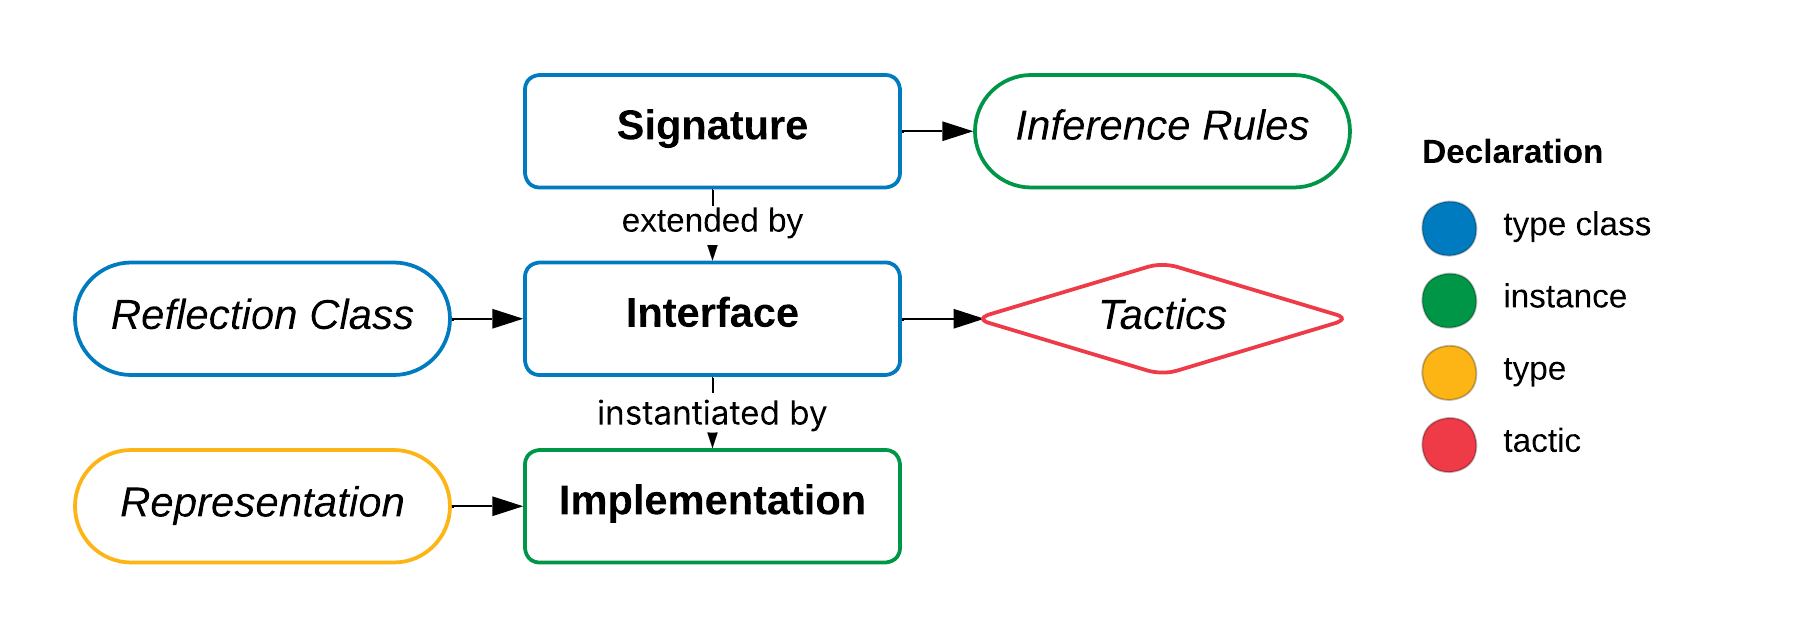
\includegraphics[width=5in]{architecture.png}
\end{figure}

\begin{figure}
\centering
\caption{The inference procedure constructs an upper bound on the degree of a polynomial.}
\label{fig:inference}
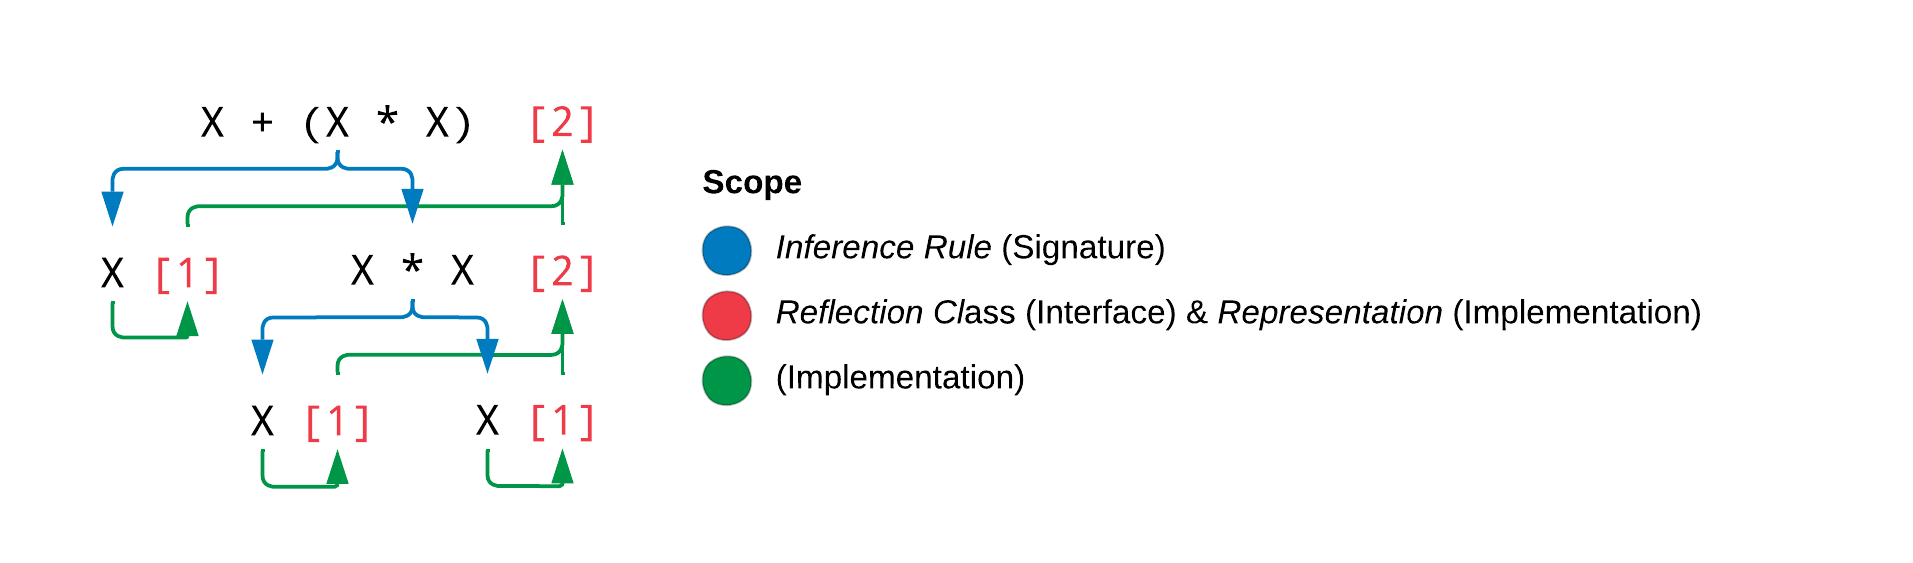
\includegraphics[width=6in]{inference.png}
\end{figure}

\secb{Sensitive Inference Procedure}
\label{sec:sensitive}

Although the inference procedure is effective for target properties with inference rules that require only the simple input instances without extra conditions, it is limited for properties that require extra assumptions at each step. For example, inference for exact degrees and leading coefficients requires that leading terms do not cancel at each \leaninline{+}, \leaninline{*}, or \leaninline{\^{}} step. To address this issue, we implement the \emph{sensitive inference procedure} which is invoked by Tactic~\ref{tac:infer_instance_trying}.

\begin{tactic}[\tacticinline{infer\_instance\_trying}]
\label{tac:infer_instance_trying}
\lean{Lean.MVarId.synthInstanceTrying, «tacticInfer_instance_trying<:>_»}
\leanok
Performs a depth-first search which, at each step, applies a provided helper tactic \tacticinline{t} then checks all instance declarations that match the current goal. Unlike Lean's type-class inference, this procedure supports instance declarations that require assumptions that cannot be resolved by type-class instances, handling them with the helper tactic instead. The syntax is \tacticinline{infer\_instance\_trying}\leaninline{ <:> }\tacticinline{t}.
\begin{lstlisting}
open Nat

class IsDouble (n : ℕ) where
  m : ℕ
  h : n = 2 * m

instance (h : n % 2 = 0) : IsDouble n :=
  ⟨n / 2, (Nat.mul_div_cancel' (dvd_of_mod_eq_zero h)).symm⟩

example : IsDouble 4 := by infer_instance_trying <:> decide
\end{lstlisting}
\end{tactic}

\seca{Univariate System}
\label{sec:univariate}

\secb{Inference Rules}

We define type classes that declare groups of inference rules. These classes may be extended to construct specifications for inference procedures requiring assumptions of varying strenghts (e.g. from nonsensitive to very sensitive). An implementation of an inference procudure must meet its specificaitions by implementing its inference rules.

Because we differentiate between inference rules for bases cases and inference rules for recursive cases of polynomials, inference procedures may be sensitive to varying degrees. To demonstrate:

\begin{itemize}
\item \textbf{Nonsensitive}: greedy degree upper bound inference is nonsensitive as it never requires additional assumptions beyond the input instances
\item \textbf{Somewhat sensitive}: leading coefficient inference is sensitive in recursive cases but nonsensitive in base cases
\item \textbf{Very sensitive}: exact degree inference is sensitive as it always requires additional assumptions beyond the input instances
\end{itemize}

It should also be emphasized that when we assert that we require some type in the following definitions, we mean that we must be provided a way to compute a member of that type, not just that such a member exists, given the current assumptions as input.

\begin{definition}[Nonsensitive rules for base cases]
\label{def:BaseReflection}
\lean{Polynomial.Rfl.BaseReflection}
\leanok
Given a semiring $R$ and a property of polynomials $T:R[x] \to \mathtt{Type}$, nonsensitive inference of $T$ for base cases of $R[x]$ requires that we have the following.
\begin{itemize}
\item $T(0)$
\item $T(c)$ for $c \in R$
\item $T(x)$
\item $T(x ^ n)$ for $n \in \mathbb{N}$
\end{itemize}
The $T(x ^ n)$ case is not strictly necessary here and could have been analyzed as a result of recursive cases. However, $T(x ^ n)$ often has a nice closed form so it is included here for efficiency.
\end{definition}

\begin{definition}[Nonsensitive rules for recursive cases]
\label{def:ClosureReflection}
\lean{Polynomial.Rfl.ClosureReflection}
\leanok
Given a semiring $R$ and a property of polynomials $T:R[x] \to \mathtt{Type}$, nonsensitive inference of $T$ for recursive cases of $R[x]$ requires that we have the following.
\begin{itemize}
\item $T(p^n)$ given $T(p)$ for $p \in R[x]$ and $n \in \mathbb{N}$
\item $T(pq)$ given $T(p)$ and $T(q)$ for $p,q \in R[x]$
\item $T(p+q)$ given $T(p)$ and $T(q)$ for $p,q \in R[x]$
\end{itemize}
\end{definition}

\begin{definition}[Sensitive rules for base cases]
\label{def:SensitiveBaseReflection}
\lean{Polynomial.Rfl.SensitiveBaseReflection}
\leanok
Given a semiring $R$ and a property of polynomials $T:R[x] \to \mathtt{Type}$, sensitive inference of $T$ for base cases of $R[x]$ requires that we have the following.
\begin{itemize}
\item $T(0)$
\item $T(c)$ for $c \in R \setminus \{0\}$
\item $T(x)$ when $R$ is nontrivial
\item and $T(x ^ n)$ for $n \in \mathbb{N}$ when $R$ is nontrivial
\end{itemize}
The $T(x ^ n)$ case is not strictly necessary here and could have been analyzed as a result of recursive cases. However, $T(x ^ n)$ often has a nice closed form so so it is included here for efficiency.
\end{definition}

\begin{definition}[Sensitive rules for recursive cases]
\label{def:SensitiveClosureReflection}
\lean{Polynomial.Rfl.SensitiveClosureReflection}
\leanok
Given a semiring $R$ and a property of polynomials $T:R[x] \to \mathtt{Type}$, sensitive inference of $T$ for recursive cases of $R[x]$ requires that we have the following.
\begin{itemize}
\item $T(p^n)$ given $T(p)$ for $p \in R[x]$ and $n \in \mathbb{N}$ when $\leading(p^n) \neq 0$
\item $T(pq)$ given $T(p)$ and $T(q)$ for $p,q \in R[x]$ when $\leading(p)\leading(q) \neq 0$
\item $T(p+q)$ given $T(p)$ for $p,q \in R[x]$ when $\degree(p) > \degree(q)$
\item $T(p+q)$ given $T(q)$ for $p,q \in R[x]$ when $\degree(p) < \degree(q)$
\item $T(p+q)$ given $T(p)$ and $T(q)$ for $p,q \in R[x]$ when $\degree(p) = \degree(q)$ and $\leading(p) + \leading(q) \neq 0$
\end{itemize}
\end{definition}

Many useful representations have a simplified or normal form when different members of that representation are equivalent up to the target property. For instance, lists of polynomial coefficients are equivalent up to trailing zeros and can typically be simplified to an equivalent normal form with no trailing zeros. In this case, degrees and leading coefficients are easily computed from a normal form, which is reflected in Definition~\ref{def:NormalizerReflection}.

\begin{definition}[Type with a normal form]
\label{def:Normalizer}
\lean{Normalizer}
\leanok
We say that a type $t$ has a normal form if there is a set $N \subseteq \{m:t\}$ and an idempotent function $f:t \to N$. Let $m : t$. $m$ is called \emph{normal} if $m \in N$. $f(m)$ is called the \emph{normalization} of $m$.
\end{definition}

\begin{definition}[Rules for representations with a normal form]
\label{def:NormalizerReflection}
\lean{Polynomial.Rfl.NormalizerReflection}
\leanok
\uses{def:Normalizer}
Given a semiring $R$ and a property of polynomials $T:R[x] \to \mathtt{Type}$, inference of $T$ for representations with a normal form requires that we have the following when equality in $R$ is decidable.
\begin{itemize}
\item a normal form for $T(p)$ for $p \in R[x]$
\item \leaninline{DegreeEq}$(p)$ given a normal $T(p)$ for $p \in R[x]$
\item \leaninline{LeadingCoeff}$(p)$ given a normal $T(p)$ for $p \in R[x]$
\end{itemize}
\end{definition}

It is also often useful to rewrite a polynomial in a standard form defined by the representation, such as with expanded and ordered terms for example.

\begin{definition}[Rules for representations that support rewriting in a standard form]
\label{def:FormReflection}
\lean{Polynomial.Rfl.FormReflection}
\leanok
Given a semiring $R[x]$ and a property of polynomials $T:R[x] \to \mathtt{Type}$, inference of $T$ for representations that support rewriting to a standard form requires the following.
\begin{itemize}
\item $q \in R[x]$ given $T(p)$ for $p \in R[x]$ such that $q = p$
\end{itemize}
\end{definition}

\secb{Reflection Classes}

TODO

\secb{Representations}

TODO

\secb{Tactics}
\label{sec:tactics}

\secc{Utility tactics}

Utility tactics perform useful rewriting and last-mile simplification steps. They appear frequently in those reflection tactics that perform the inference procedure.

\begin{tactic}[\tacticinline{poly\_rfl\_rw}]
\label{tac:poly_rfl_rw}
\lean{tacticPoly_rfl_rw}
\leanok
Performs trivial rewrites to transform polynomials into the form expected by the inference procedure. For instance, \leaninline{0} is rewritten as \leaninline{C 0}.
\end{tactic}

\begin{tactic}[\tacticinline{poly\_rfl\_dsimp}]
\label{tac:poly_rfl_dsimp}
\lean{tacticPoly_rfl_dsimp}
\leanok
\uses{def:NormalizerReflection, def:FormReflection}
Simplifies the expression resulting from the inference procedure so that the computable representation is visible. This consists primarily of unfolding reflection class instances into the values they contain.
\end{tactic}

\begin{tactic}[\tacticinline{poly\_rfl\_with}]
\label{tac:poly_rfl_with}
\lean{«tacticPoly_rfl_with<:>_»}
\leanok
\uses{tac:poly_rfl_rw, tac:poly_rfl_dsimp}
Frames a reflection tactic \tacticinline{t} with rewriting and last-mile simplification steps from Tactic~\ref{tac:poly_rfl_rw} and Tactic~\ref{tac:poly_rfl_dsimp}. The syntax is \tacticinline{poly\_rfl\_with}\leaninline{ <:> }\tacticinline{t}.
\end{tactic}

\begin{tactic}[\tacticinline{poly\_infer\_try}]
\label{tac:poly_infer_try}
\lean{tacticPoly_infer_try}
\leanok
\uses{tac:poly_rfl_dsimp}
For use as a helper tactic in the sensitive inference procedure (see Tactic~\ref{tac:infer_instance_trying}). Invokes Tactic~\ref{tac:poly_rfl_dsimp} to unfold the expression resulting from the previous step of the sensitive inference procedure, preparing the goal for the next step.
\end{tactic}

\secc{Reflection tactics}

Reflection tactics perform the inference procedure to resolve target goals by transforming them so that they can be resolved with last-mile automation tactics such as \tacticinline{trivial}, \tacticinline{simp}, and \tacticinline{norm\_num}. The code samples are adapted from \href{https://github.com/LiamSchilling/AutomatePolynomial/tree/master/AutomatePolynomial/Demo/Polynomial.lean}{\texttt{Demo/Polynomial.lean}} and rely on the following preamble.

\begin{lstlisting}
import AutomatePolynomial.Reflection.Polynomial.Basic
open Polynomial Rfl
\end{lstlisting}

\begin{tactic}[\tacticinline{poly\_rfl\_degree\_le}]
\label{tac:poly_rfl_degree_le}
\lean{tacticPoly_rfl_degree_le}
\leanok
\uses{tac:poly_rfl_with}
Resolves goals of the form $\degree(p) \leq n$ for univariate polynomials $p$ and some $n$ which is either a natural number or the bottom member $\bot$.
\begin{lstlisting}
section DegreeLe
variable [Semiring R]
example : (0     : R[X]).degree ≤ ⊥ := by poly_rfl_degree_le; trivial
example : (1     : R[X]).degree ≤ 0 := by poly_rfl_degree_le; trivial
example : (X     : R[X]).degree ≤ 1 := by poly_rfl_degree_le; trivial
example : (X ^ 2 : R[X]).degree ≤ 2 := by poly_rfl_degree_le; trivial
example : (X + 1 : R[X]).degree ≤ 1 := by poly_rfl_degree_le; trivial
end DegreeLe
\end{lstlisting}
\end{tactic}

Since the following tactics deal with properties that depend on whether leading terms cancel---degrees and leading coefficients---they will rely on the sensitive inference procedure (see Section~\ref{sec:sensitive}) in cases where the polynomial contains recursive cases such as \leaninline{+}, \leaninline{*}, or \leaninline{\^{}} (disregarding \leaninline{X \^{} n} which is handled separately). Tactics with the suffix \tacticinline{\_trying} perform the sensitive inference procedure to handle these cases. Alternatively, the sensitive inference procedure may be avoided by instead infering the coefficients of the polynomial and then deriving the target property from that. Tactics with the suffix \tacticinline{\_of\_coeffs} use this alternative when provided the the target representation of the coefficients, such as \leaninline{CoeffsList}.

\begin{tactic}[\tacticinline{poly\_rfl\_degree\_eq}]
\label{tac:poly_rfl_degree_eq}
\lean{tacticPoly_rfl_degree_eq, «tacticPoly_rfl_degree_eq_trying<:>_», tacticPoly_rfl_degree_eq_of_coeffsVIA_}
\leanok
\uses{tac:poly_rfl_with}
Resolves goals of the form $\degree(p) = n$ for univariate polynomials $p$ and some $n$ which is either a natural number or the bottom member $\bot$. In any case where we want $\degree(p) \neq \bot$, we must admit that the the semiring is nontrivial, as in section \leaninline{DegreeEqNontrivial}.
\begin{lstlisting}
section DegreeEq
variable [Semiring R]
example : (0 : R[X]).degree = ⊥ := by poly_rfl_degree_eq
end DegreeEq

section DegreeEqNontrivial
variable [Semiring R] [Nontrivial R]
example : (1     : R[X]).degree = 0 := by poly_rfl_degree_eq
example : (X     : R[X]).degree = 1 := by poly_rfl_degree_eq
example : (X ^ 2 : R[X]).degree = 2 := by poly_rfl_degree_eq
example : (X + 1 : R[X]).degree = 1 := by poly_rfl_degree_eq_trying <:> poly_infer_try
end DegreeEqNontrivial

section DegreeEqOfCoeffs
example : (X + 1 : ℕ[X]).degree = 1 := by poly_rfl_degree_eq_of_coeffs VIA CoeffsList; simp; trivial
end DegreeEqOfCoeffs
\end{lstlisting}
\end{tactic}

\begin{tactic}[\tacticinline{poly\_rfl\_leading\_coeff}]
\label{tac:poly_rfl_leading_coeff}
\lean{tacticPoly_rfl_leading_coeff, «tacticPoly_rfl_leading_coeff_trying<:>_», tacticPoly_rfl_leading_coeff_of_coeffsVIA_}
\leanok
\uses{tac:poly_rfl_with}
Resolves goals of the form $\leading(p) = c$ for univariate polynomials $p$ and members of the relevant semiring $c$. When the definition of $p$ contains recursive cases such as \leaninline{+}, \leaninline{*}, or \leaninline{\^{}} (disregarding \leaninline{X \^{} n} which is handled separately), we must admit that the semiring is nontrivial, as in section \leaninline{LeadingCoeffNontrivial}.
\begin{lstlisting}
section LeadingCoeff
variable [Semiring R]
example : (0     : R[X]).leadingCoeff = 0 := by poly_rfl_leading_coeff
example : (1     : R[X]).leadingCoeff = 1 := by poly_rfl_leading_coeff
example : (X     : R[X]).leadingCoeff = 1 := by poly_rfl_leading_coeff
example : (X ^ 2 : R[X]).leadingCoeff = 1 := by poly_rfl_leading_coeff
end LeadingCoeff

section LeadingCoeffNontrivial
variable [Semiring R] [Nontrivial R]
example : (X + 1 : R[X]).leadingCoeff = 1 := by poly_rfl_leading_coeff_trying <:> poly_infer_try
end LeadingCoeffNontrivial

section LeadingCoeffEqOfCoeffs
example : (X + 1 : ℕ[X]).leadingCoeff = 1 := by poly_rfl_leading_coeff_of_coeffs VIA CoeffsList; simp
end LeadingCoeffEqOfCoeffs
\end{lstlisting}
\end{tactic}

The remaining tactics are generic to the representation of the target property and require the user to provide the target representation, such as \leaninline{CoeffsList} or \leaninline{EvalArrow}.

\begin{tactic}[\tacticinline{poly\_rfl\_coeff}]
\label{tac:poly_rfl_coeff}
\lean{tacticPoly_rfl_coeffVIA_}
\leanok
\uses{tac:poly_rfl_with}
Resolves goals of the form $\coeff_n(p) = c$ for univariate polynomials $p$, natural numbers $n$, and members of the relevant semiring $c$. Note that we admit that the semiring is commutative.
\begin{lstlisting}
section Coeffs
variable [CommSemiring R]
example : (0     : R[X]).coeff 1 = 0 := by poly_rfl_coeff VIA CoeffsList
example : (1     : R[X]).coeff 1 = 0 := by poly_rfl_coeff VIA CoeffsList; trivial
example : (X     : R[X]).coeff 1 = 1 := by poly_rfl_coeff VIA CoeffsList; trivial
example : (X ^ 2 : R[X]).coeff 1 = 0 := by poly_rfl_coeff VIA CoeffsList; trivial
example : (X + 1 : R[X]).coeff 1 = 1 := by poly_rfl_coeff VIA CoeffsList; simp
end Coeffs
\end{lstlisting}
\end{tactic}

\begin{tactic}[\tacticinline{poly\_rfl\_eval}]
\label{tac:poly_rfl_eval}
\lean{tacticPoly_rfl_evalVIA_}
\leanok
\uses{tac:poly_rfl_with}
Resolves goals of the form $p(c) = c'$ for univariate polynomials $p$ and members of the relevant semiring $c$ and $c'$. Note that we admit that the semiring is commutative.
\begin{lstlisting}
section Eval
variable [CommSemiring R]
example : (0     : R[X]).eval 1 = 0 := by poly_rfl_eval VIA EvalArrow
example : (1     : R[X]).eval 1 = 1 := by poly_rfl_eval VIA EvalArrow
example : (X     : R[X]).eval 1 = 1 := by poly_rfl_eval VIA EvalArrow
example : (X ^ 2 : R[X]).eval 1 = 1 := by poly_rfl_eval VIA EvalArrow; simp
example : (X + 1 : R[X]).eval 1 = 2 := by poly_rfl_eval VIA EvalArrow; norm_num
end Eval
\end{lstlisting}
\end{tactic}

\begin{tactic}[\tacticinline{poly\_rfl\_expand}]
\label{tac:poly_rfl_expand}
\lean{tacticPoly_rfl_expandVIA_}
\leanok
\uses{tac:poly_rfl_with, def:FormReflection}
Resolves goals of the form $p = q$ for a univariate polynomial $p$ and an equivalent polynomial $q$ in expanded form. Note that we admit that the semiring is commutative.
\begin{lstlisting}
section Expand
variable [CommSemiring R]
example : (C 2 + X : R[X]) = X + C 2 := by poly_rfl_expand VIA CoeffsList; simp; poly_unfold_expand; simp
example : (X * C 2 : R[X]) = C 2 * X := by poly_rfl_expand VIA CoeffsList; simp; poly_unfold_expand; simp
example : (X + X   : R[X]) = C 2 * X := by poly_rfl_expand VIA CoeffsList; simp; poly_unfold_expand; norm_num
end Expand
\end{lstlisting}
\end{tactic}

\seca{Multivariate System}
\label{sec:multivariate}

Current work focuses on generalizing the capabilities of the system for univariate polynomials to a system for multivariate polynomials. Progress on this system is available in the \href{https://github.com/LiamSchilling/AutomatePolynomial/tree/feature/mvpoly}{\texttt{feature/mvpoly}} branch.

\newpage
\bibliography{refs}

\end{document}

\home{https://LiamSchilling.github.io/AutomatePolynomial}
\github{https://github.com/LiamSchilling/AutomatePolynomial}
\dochome{https://LiamSchilling.github.io/AutomatePolynomial/docs}

\title{AutomatePolynomial: An Experiment in Reflection for Polynomials}
\author{Liam Schilling \and Quang Dao}

\begin{document}
\maketitle
\seca*{Abstract}
Polynomials are crucial to cryptographic protocols for their error-checking applications. Proof assistants like Lean 4 enable machine-verified implementations of those protocols, yielding more correct and secure systems. While those implementations demand an efficient way to prove properties of polynomials in Lean, representations of polynomials in Lean’s mathematics library are not directly computable, making simple results tedious to prove. To address this issue, we design and implement a general proof-by-reflection model in Lean, reducing mathematical problems to decisions on computable representations.

The resulting systems automate proof of degrees, coefficients, evaluations, and expansions for univariate and multivariate polynomials in various contexts. The model’s design specifies three levels of abstraction, producing modular and reusable tactics that are generic to computable representations of properties. We demonstrate this by exploring representations such as lambda functions for evaluations, dense lists for univariate coefficients, and dense trees for multivariate coefficients. Sparse and array representations are priorities for future work to improve efficiency. This work provides automated proving tools for polynomials and a general proof-by-reflection model for Lean, contributing to the development of reliable, machine-verified systems.

% In this file you should put the actual content of the blueprint.
% It will be used both by the web and the print version.
% It should *not* include the \begin{document}
%
% If you want to split the blueprint content into several files then
% the current file can be a simple sequence of \input. Otherwise It
% can start with a \section or \chapter for instance.

\seca{Introduction}
\label{sec:intro}

\secb{Organization of the Blueprint}

The blueprint is organized as follows: The rest of Section~\ref{sec:intro} examines previous work in proof automation and polynomials in Lean, and provides a brief comparison with the approach taken in our work. Section~\ref{sec:reflection} describes our approach to proof by reflection and outlines a model for its implementation. This section will also be of interest to readers curious about our use of type-class inference in proof automation. Section~\ref{sec:univariate} details the implementation of each part of the model for univariate polynomials. Readers interested in using the univariate system for proof automation should be directed specifially to Section~\ref{sec:tactics}. Section~\ref{sec:multivariate} addresses ongoing work towards a system for multivariate polynomials.

\secb{Automation in Lean}
\label{sec:automation}

Previous work outlines a number of approaches to proof automation in Lean 4, each with different advantages and preferred applications. The Ring of Integers project \cite{RingOfIntegers2025} covers proof automation methods in Lean extensively and may be referenced for a more technical address of the topic. This blueprint will introduce and evaluate proof automation strategies in previous work as it relates to our approach. We broadly refer to these strategies as \emph{proof by reflection}.

One proof-by-reflection paradigm is white-box automation \cite{Aesop2023}, in which the automation procedure is transparent and simple enough for users to trace and predict how an application will deal with their goals. Although these solutions tend to be narrow-application in terms of the goals they can deal with, they are highly extensible to different contexts since the user can understand and customize them. Search tactics such as \tacticinline{aesop} \cite{Aesop2023} and reflection models such as LeanSSR \cite{SmallScaleReflection2024} are common examples of such automation. While alternative proof-by-reflection paradigms such as LLMs are more general-application, they tend to be more brittle to changes in context and difficult to debug due to their complexity. There have even been recent efforts to make these solutions more usable by integrating them as assistants in the interactive-proving process, using them to resolve subgoals instead of relying on them for complex theorems. Lean Copilot \cite{LeanCopilot2025}, for instance, integrates their LLM implementation with aesop’s search, resulting in a white-box solution with some of the general-application benefits of LLM automation.

Popular implementations also tend to be native to Lean since they are easier to use, entail less dependencies, and enjoy the benefits of Lean's powerful tactics and metaprogramming. For instance, Lean Copilot \cite{LeanCopilot2025} implements their Lean declarations in C++, to which Lean compiles directly. Moreover, LeanSSR \cite{SmallScaleReflection2024} emphasizes how Lean is a great candidate for implementation of their reflection model because of its powerful metaprogramming support. LeanSSR also discusses how Lean's flexible tactics for goal manipulation result in convenient ``last-mile automation'' strategies, where the user only needs to manipulate the goal to a point where it can be automatically resolved by some form of reduction. For example, the built-in tactics \tacticinline{rfl} and \tacticinline{simp} automate a variety of goals by reducing them according to simple rules. Our native approach makes generous use of these last-mile automation strategies. Overall, it seems that native, white-box automation is a leading contender for Lean.

Type-class inference, which our project employs to construct computable representations, seems unexplored as a search method compared to metaprogramming and search tactics. We find in our project that it greatly simplifies resolving goals that can be split into similar subgoals without much additional verification at each step. However, it requires additional help from tactics when verification beyond the scope of the procedure is necessary at any step (see Section~\ref{sec:sensitive}).

\secb{Polynomials in Lean}

Previous work with polynomials in Lean highlights how a lack of computable representations can limit the impact of a formalization. As described by Wieser \cite{ComputationalPolynomialsFinsupps}, polynomials in Mathlib are non-computable because they are implemented using the \leaninline{Finsupp} type for finitely supported functions, whose underlying support set may not have decidable membership. An early Lean 3 formalization \cite{MasonStothers2018} aimed to prove the Mason Stothers Theorem. The project achieved this goals, though it first had to build up the necessary background in number theory and polynomials. A later project \cite{MasonStothers2024} which achieved the same formalization using Lean 4’s Mathlib noted that the previous project’s rejection of established machinery limited its application and reusability. This is because its results cannot be easily related to the standard Mathlib definitions used in other projects.

Some projects take advantage of the computational benefits of machine formalization, implementing algorithms on polynomials in Lean. One project implemented Buchberger’s Algorithm \cite{Buchbergers2019} but noted that Mathlib’s non-computable polynomial representation made it ineffective for their application. The authors implemented their own polynomials for use in their implementation, limiting its reusability similarly to the projects dealing with the Mason Stothers Theorem. Another project \cite{UnivariateSolutions2022} implemented algorithms for finding solutions to univariate polynomials, but built their mathematical machinery---all the way from natural numbers---from scratch. Although an impressive look into what it takes to formalize such mathematical background, this definitional separation limits the project in the same ways as the previous one.

Recent work focuses on more computable representations and automations for polynomials in Lean. Davenport \cite{ComputationalPolynomials2024} outlines the design decisions towards implementing such a representation and some operations on it. However, he does not detail any proof of correctness for those operations, and instead discusses verification using SageMath. Another approach to automation is Wieser’s \tacticinline{polyrith} tactic \cite{Polyrith}, which uses SageMath to compute necessary parameters for resolving a goal with Mathlib’s \tacticinline{linear\_combination} tactic. It is a highly effective white-box method for polynomials over fields. In both these methods, proof automation is non-native. Our approach introduces a computable representation and correctness-verified operations all native to Lean. Furthermore, the representations do not require polynomials defined over fields, only commutative semirings in the most specific cases, making the solution more general than polyrith in this aspect.

The Ring of Integers project \cite{RingOfIntegers2025} briefly discusses construction of computable representations based on expressions in the current goal as a proof automation method. They also discuss their list-based implementation of a computable representation for polynomials which is similar to our list-based implementation. However, they explain as a limitation that their implementation does not provide such a way to automatically construct this representation. This type of automated construction is central to our approach and is achieved using the unexplored method of type-class inference (recall Section~\ref{sec:automation}). For these reasons, we consider this aspect the most novel contribution of our work.

It should be noted that the powerful \tacticinline{grind} tactic \cite{Grind} for automated reasoning over finite algebras became available in Lean during work on this project. For its Gröbner basis computations, the system ships with a computable representation of polynomials implemented by the \leaninline{Poly} type (see \href{https://github.com/leanprover/lean4/blob/master/src/Init/Grind/Ring/Poly.lean}{\texttt{Poly.lean}}) and automated construction methods for it. It is still unclear how those automated construction methods compare to those used in our project, though future work may explore this question as well as how adoption of the convenient \leaninline{Poly} type could improve our system.

\seca{Reflection by Inference}
\label{sec:reflection}

\secb{Representation Inference}

Lean's type-class inference is a powerful tool for automatically constructing instances of a parameterized type. Our approach to proof-by-reflection, which we will call \emph{reflection by inference}, employs type-class inference to construct computable representations of target properties. First, we will briefly discuss type-class inference. Instance declarations are the blueprint for this process; each declaration states the parameter of the type it instantiates, admits any type class instances it requires as input, and specifies how to construct the target instance from these inputs. As displayed in Figure~\ref{fig:inference}, type-class inference is a depth-first search which, at each step, checks all instance declarations that match the current goal. For more details on type-class inference, consult the \textit{Theorem Proving in Lean 4} handbook \cite{TypeClasses}.

Lean's type-class inference is central to our reflection model and we will refer to it as the \emph{inference procedure}. In our case, the types we will construct are of computable representations of the target properties parameterized over polynomials. We will refer to these computable representions as \emph{representations} and the type classes that contain instances of them as \emph{reflection classes}. As addressed in Figure~\ref{fig:model}, reflection classes are generic to the representations they contain. It follows that the inference procedure is generic to computable representations of the target properties. We will refer to instance declarations for reflection classes as \emph{inference rules}. Once the reflection classes and inference rules are declared, we may implement \emph{tactics} that perform the inference procedure to resolve goals. These tactics rewrite the target property as the constructed computable representation so that the goal can be resolved by last-mile automation tactics. Recall that the LeanSSR project \cite{SmallScaleReflection2024} discusses last-mile automation.

\secb{Reflection Model}

The reflection-by-inference model in Figure~\ref{fig:model} guides our implementation of the system for polynomials. We ensure levels of modularity with respect to the target property and the representation of that property by specifying three levels of abstraction: The \emph{signature} declares inference rules for generic reflection classes. The \emph{interface} extends multiple signatures with a specified reflection class that asserts the target property. At this level, tactics may be implemented for generic representations. The \emph{implementation} instantiates an interface with a specified representation of the target property and implements the rules declared in the signatures.

\begin{figure}
\centering
\caption{Visualization of the reflection-by-inference model.}
\label{fig:model}
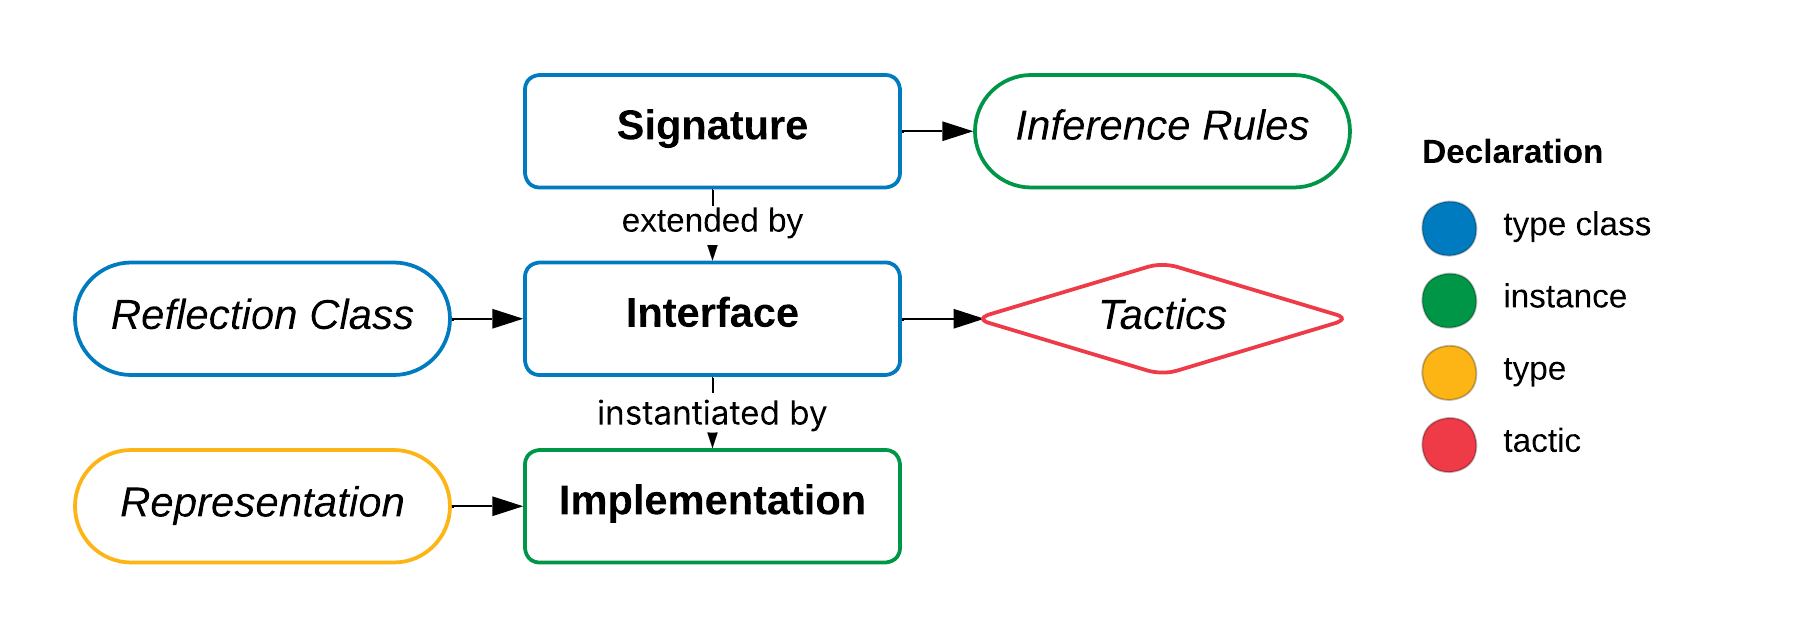
\includegraphics[width=5in]{architecture.png}
\end{figure}

\begin{figure}
\centering
\caption{The inference procedure constructs an upper bound on the degree of a polynomial.}
\label{fig:inference}
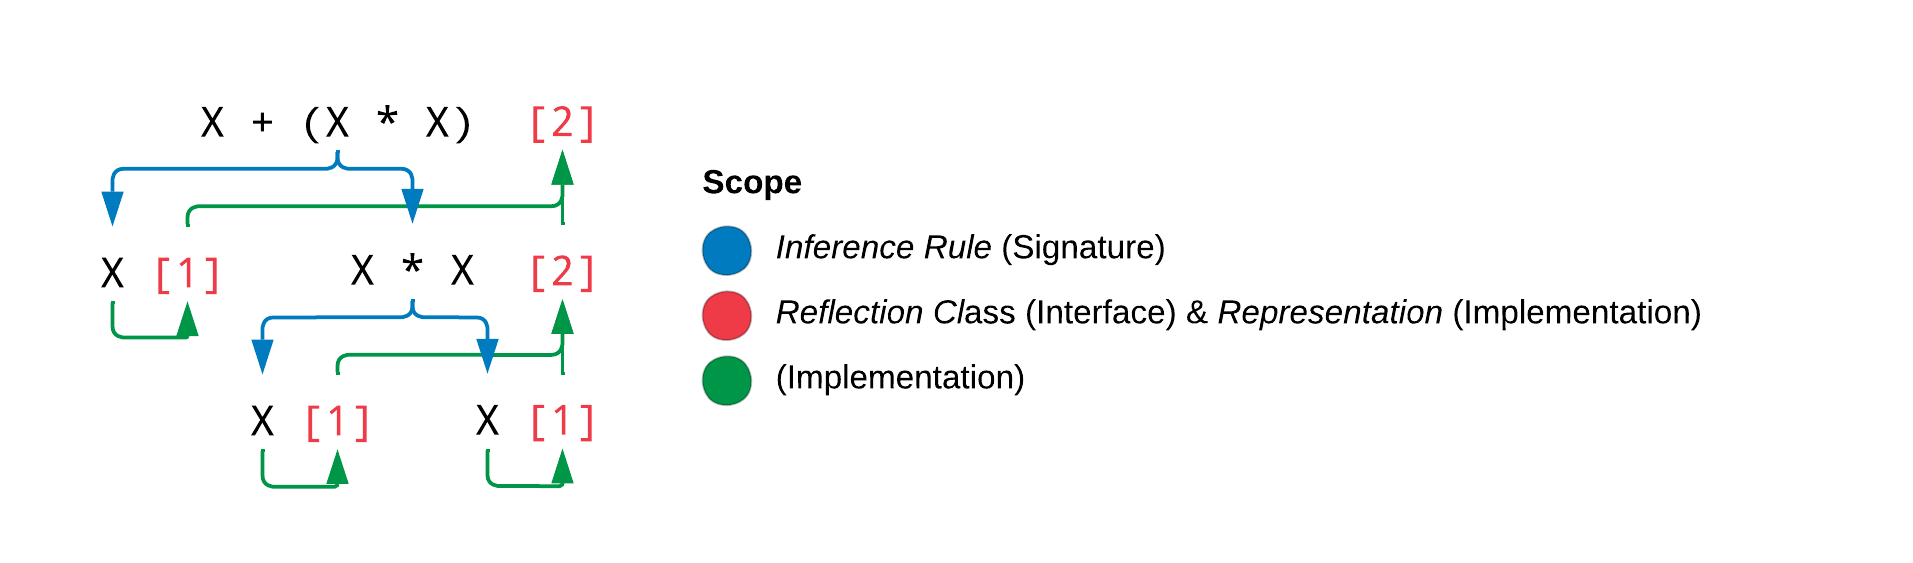
\includegraphics[width=6in]{inference.png}
\end{figure}

\secb{Sensitive Inference Procedure}
\label{sec:sensitive}

Although the inference procedure is effective for target properties with inference rules that require only the simple input instances without extra conditions, it is limited for properties that require extra assumptions at each step. For example, inference for exact degrees and leading coefficients requires that leading terms do not cancel at each \leaninline{+}, \leaninline{*}, or \leaninline{\^{}} step. To address this issue, we implement the \emph{sensitive inference procedure} which is invoked by Tactic~\ref{tac:infer_instance_trying}.

\begin{tactic}[\tacticinline{infer\_instance\_trying}]
\label{tac:infer_instance_trying}
\lean{Lean.MVarId.synthInstanceTrying, «tacticInfer_instance_trying<:>_»}
\leanok
Performs a depth-first search which, at each step, applies a provided helper tactic \tacticinline{t} then checks all instance declarations that match the current goal. Unlike Lean's type-class inference, this procedure supports instance declarations that require assumptions that cannot be resolved by type-class instances, handling them with the helper tactic instead. The syntax is \tacticinline{infer\_instance\_trying}\leaninline{ <:> }\tacticinline{t}.
\begin{lstlisting}
open Nat

class IsDouble (n : ℕ) where
  m : ℕ
  h : n = 2 * m

instance (h : n % 2 = 0) : IsDouble n :=
  ⟨n / 2, (Nat.mul_div_cancel' (dvd_of_mod_eq_zero h)).symm⟩

example : IsDouble 4 := by infer_instance_trying <:> decide
\end{lstlisting}
\end{tactic}

\seca{Univariate System}
\label{sec:univariate}

\secb{Inference Rules}

We define type classes that declare groups of inference rules. These classes may be extended to construct specifications for inference procedures requiring assumptions of varying strenghts (e.g. from nonsensitive to very sensitive). An implementation of an inference procudure must meet its specificaitions by implementing its inference rules.

Because we differentiate between inference rules for bases cases and inference rules for recursive cases of polynomials, inference procedures may be sensitive to varying degrees. To demonstrate:

\begin{itemize}
\item \textbf{Nonsensitive}: greedy degree upper bound inference is nonsensitive as it never requires additional assumptions beyond the input instances
\item \textbf{Somewhat sensitive}: leading coefficient inference is sensitive in recursive cases but nonsensitive in base cases
\item \textbf{Very sensitive}: exact degree inference is sensitive as it always requires additional assumptions beyond the input instances
\end{itemize}

It should also be emphasized that when we assert that we require some type in the following definitions, we mean that we must be provided a way to compute a member of that type, not just that such a member exists, given the current assumptions as input.

\begin{definition}[Nonsensitive rules for base cases]
\label{def:BaseReflection}
\lean{Polynomial.Rfl.BaseReflection}
\leanok
Given a semiring $R$ and a property of polynomials $T:R[x] \to \mathtt{Type}$, nonsensitive inference of $T$ for base cases of $R[x]$ requires that we have the following.
\begin{itemize}
\item $T(0)$
\item $T(c)$ for $c \in R$
\item $T(x)$
\item $T(x ^ n)$ for $n \in \mathbb{N}$
\end{itemize}
The $T(x ^ n)$ case is not strictly necessary here and could have been analyzed as a result of recursive cases. However, $T(x ^ n)$ often has a nice closed form so it is included here for efficiency.
\end{definition}

\begin{definition}[Nonsensitive rules for recursive cases]
\label{def:ClosureReflection}
\lean{Polynomial.Rfl.ClosureReflection}
\leanok
Given a semiring $R$ and a property of polynomials $T:R[x] \to \mathtt{Type}$, nonsensitive inference of $T$ for recursive cases of $R[x]$ requires that we have the following.
\begin{itemize}
\item $T(p^n)$ given $T(p)$ for $p \in R[x]$ and $n \in \mathbb{N}$
\item $T(pq)$ given $T(p)$ and $T(q)$ for $p,q \in R[x]$
\item $T(p+q)$ given $T(p)$ and $T(q)$ for $p,q \in R[x]$
\end{itemize}
\end{definition}

\begin{definition}[Sensitive rules for base cases]
\label{def:SensitiveBaseReflection}
\lean{Polynomial.Rfl.SensitiveBaseReflection}
\leanok
Given a semiring $R$ and a property of polynomials $T:R[x] \to \mathtt{Type}$, sensitive inference of $T$ for base cases of $R[x]$ requires that we have the following.
\begin{itemize}
\item $T(0)$
\item $T(c)$ for $c \in R \setminus \{0\}$
\item $T(x)$ when $R$ is nontrivial
\item and $T(x ^ n)$ for $n \in \mathbb{N}$ when $R$ is nontrivial
\end{itemize}
The $T(x ^ n)$ case is not strictly necessary here and could have been analyzed as a result of recursive cases. However, $T(x ^ n)$ often has a nice closed form so so it is included here for efficiency.
\end{definition}

\begin{definition}[Sensitive rules for recursive cases]
\label{def:SensitiveClosureReflection}
\lean{Polynomial.Rfl.SensitiveClosureReflection}
\leanok
Given a semiring $R$ and a property of polynomials $T:R[x] \to \mathtt{Type}$, sensitive inference of $T$ for recursive cases of $R[x]$ requires that we have the following.
\begin{itemize}
\item $T(p^n)$ given $T(p)$ for $p \in R[x]$ and $n \in \mathbb{N}$ when $\leading(p^n) \neq 0$
\item $T(pq)$ given $T(p)$ and $T(q)$ for $p,q \in R[x]$ when $\leading(p)\leading(q) \neq 0$
\item $T(p+q)$ given $T(p)$ for $p,q \in R[x]$ when $\degree(p) > \degree(q)$
\item $T(p+q)$ given $T(q)$ for $p,q \in R[x]$ when $\degree(p) < \degree(q)$
\item $T(p+q)$ given $T(p)$ and $T(q)$ for $p,q \in R[x]$ when $\degree(p) = \degree(q)$ and $\leading(p) + \leading(q) \neq 0$
\end{itemize}
\end{definition}

Many useful representations have a simplified or normal form when different members of that representation are equivalent up to the target property. For instance, lists of polynomial coefficients are equivalent up to trailing zeros and can typically be simplified to an equivalent normal form with no trailing zeros. In this case, degrees and leading coefficients are easily computed from a normal form, which is reflected in Definition~\ref{def:NormalizerReflection}.

\begin{definition}[Type with a normal form]
\label{def:Normalizer}
\lean{Normalizer}
\leanok
We say that a type $t$ has a normal form if there is a set $N \subseteq \{m:t\}$ and an idempotent function $f:t \to N$. Let $m : t$. $m$ is called \emph{normal} if $m \in N$. $f(m)$ is called the \emph{normalization} of $m$.
\end{definition}

\begin{definition}[Rules for representations with a normal form]
\label{def:NormalizerReflection}
\lean{Polynomial.Rfl.NormalizerReflection}
\leanok
\uses{def:Normalizer}
Given a semiring $R$ and a property of polynomials $T:R[x] \to \mathtt{Type}$, inference of $T$ for representations with a normal form requires that we have the following when equality in $R$ is decidable.
\begin{itemize}
\item a normal form for $T(p)$ for $p \in R[x]$
\item \leaninline{DegreeEq}$(p)$ given a normal $T(p)$ for $p \in R[x]$
\item \leaninline{LeadingCoeff}$(p)$ given a normal $T(p)$ for $p \in R[x]$
\end{itemize}
\end{definition}

It is also often useful to rewrite a polynomial in a standard form defined by the representation, such as with expanded and ordered terms for example.

\begin{definition}[Rules for representations that support rewriting in a standard form]
\label{def:FormReflection}
\lean{Polynomial.Rfl.FormReflection}
\leanok
Given a semiring $R[x]$ and a property of polynomials $T:R[x] \to \mathtt{Type}$, inference of $T$ for representations that support rewriting to a standard form requires the following.
\begin{itemize}
\item $q \in R[x]$ given $T(p)$ for $p \in R[x]$ such that $q = p$
\end{itemize}
\end{definition}

\secb{Reflection Classes}

TODO

\secb{Representations}

TODO

\secb{Tactics}
\label{sec:tactics}

\secc{Utility tactics}

Utility tactics perform useful rewriting and last-mile simplification steps. They appear frequently in those reflection tactics that perform the inference procedure.

\begin{tactic}[\tacticinline{poly\_rfl\_rw}]
\label{tac:poly_rfl_rw}
\lean{tacticPoly_rfl_rw}
\leanok
Performs trivial rewrites to transform polynomials into the form expected by the inference procedure. For instance, \leaninline{0} is rewritten as \leaninline{C 0}.
\end{tactic}

\begin{tactic}[\tacticinline{poly\_rfl\_dsimp}]
\label{tac:poly_rfl_dsimp}
\lean{tacticPoly_rfl_dsimp}
\leanok
\uses{def:NormalizerReflection, def:FormReflection}
Simplifies the expression resulting from the inference procedure so that the computable representation is visible. This consists primarily of unfolding reflection class instances into the values they contain.
\end{tactic}

\begin{tactic}[\tacticinline{poly\_rfl\_with}]
\label{tac:poly_rfl_with}
\lean{«tacticPoly_rfl_with<:>_»}
\leanok
\uses{tac:poly_rfl_rw, tac:poly_rfl_dsimp}
Frames a reflection tactic \tacticinline{t} with rewriting and last-mile simplification steps from Tactic~\ref{tac:poly_rfl_rw} and Tactic~\ref{tac:poly_rfl_dsimp}. The syntax is \tacticinline{poly\_rfl\_with}\leaninline{ <:> }\tacticinline{t}.
\end{tactic}

\begin{tactic}[\tacticinline{poly\_infer\_try}]
\label{tac:poly_infer_try}
\lean{tacticPoly_infer_try}
\leanok
\uses{tac:poly_rfl_dsimp}
For use as a helper tactic in the sensitive inference procedure (see Tactic~\ref{tac:infer_instance_trying}). Invokes Tactic~\ref{tac:poly_rfl_dsimp} to unfold the expression resulting from the previous step of the sensitive inference procedure, preparing the goal for the next step.
\end{tactic}

\secc{Reflection tactics}

Reflection tactics perform the inference procedure to resolve target goals by transforming them so that they can be resolved with last-mile automation tactics such as \tacticinline{trivial}, \tacticinline{simp}, and \tacticinline{norm\_num}. The code samples are adapted from \href{https://github.com/LiamSchilling/AutomatePolynomial/tree/master/AutomatePolynomial/Demo/Polynomial.lean}{\texttt{Demo/Polynomial.lean}} and rely on the following preamble.

\begin{lstlisting}
import AutomatePolynomial.Reflection.Polynomial.Basic
open Polynomial Rfl
\end{lstlisting}

\begin{tactic}[\tacticinline{poly\_rfl\_degree\_le}]
\label{tac:poly_rfl_degree_le}
\lean{tacticPoly_rfl_degree_le}
\leanok
\uses{tac:poly_rfl_with}
Resolves goals of the form $\degree(p) \leq n$ for univariate polynomials $p$ and some $n$ which is either a natural number or the bottom member $\bot$.
\begin{lstlisting}
section DegreeLe
variable [Semiring R]
example : (0     : R[X]).degree ≤ ⊥ := by poly_rfl_degree_le; trivial
example : (1     : R[X]).degree ≤ 0 := by poly_rfl_degree_le; trivial
example : (X     : R[X]).degree ≤ 1 := by poly_rfl_degree_le; trivial
example : (X ^ 2 : R[X]).degree ≤ 2 := by poly_rfl_degree_le; trivial
example : (X + 1 : R[X]).degree ≤ 1 := by poly_rfl_degree_le; trivial
end DegreeLe
\end{lstlisting}
\end{tactic}

Since the following tactics deal with properties that depend on whether leading terms cancel---degrees and leading coefficients---they will rely on the sensitive inference procedure (see Section~\ref{sec:sensitive}) in cases where the polynomial contains recursive cases such as \leaninline{+}, \leaninline{*}, or \leaninline{\^{}} (disregarding \leaninline{X \^{} n} which is handled separately). Tactics with the suffix \tacticinline{\_trying} perform the sensitive inference procedure to handle these cases. Alternatively, the sensitive inference procedure may be avoided by instead infering the coefficients of the polynomial and then deriving the target property from that. Tactics with the suffix \tacticinline{\_of\_coeffs} use this alternative when provided the the target representation of the coefficients, such as \leaninline{CoeffsList}.

\begin{tactic}[\tacticinline{poly\_rfl\_degree\_eq}]
\label{tac:poly_rfl_degree_eq}
\lean{tacticPoly_rfl_degree_eq, «tacticPoly_rfl_degree_eq_trying<:>_», tacticPoly_rfl_degree_eq_of_coeffsVIA_}
\leanok
\uses{tac:poly_rfl_with}
Resolves goals of the form $\degree(p) = n$ for univariate polynomials $p$ and some $n$ which is either a natural number or the bottom member $\bot$. In any case where we want $\degree(p) \neq \bot$, we must admit that the the semiring is nontrivial, as in section \leaninline{DegreeEqNontrivial}.
\begin{lstlisting}
section DegreeEq
variable [Semiring R]
example : (0 : R[X]).degree = ⊥ := by poly_rfl_degree_eq
end DegreeEq

section DegreeEqNontrivial
variable [Semiring R] [Nontrivial R]
example : (1     : R[X]).degree = 0 := by poly_rfl_degree_eq
example : (X     : R[X]).degree = 1 := by poly_rfl_degree_eq
example : (X ^ 2 : R[X]).degree = 2 := by poly_rfl_degree_eq
example : (X + 1 : R[X]).degree = 1 := by poly_rfl_degree_eq_trying <:> poly_infer_try
end DegreeEqNontrivial

section DegreeEqOfCoeffs
example : (X + 1 : ℕ[X]).degree = 1 := by poly_rfl_degree_eq_of_coeffs VIA CoeffsList; simp; trivial
end DegreeEqOfCoeffs
\end{lstlisting}
\end{tactic}

\begin{tactic}[\tacticinline{poly\_rfl\_leading\_coeff}]
\label{tac:poly_rfl_leading_coeff}
\lean{tacticPoly_rfl_leading_coeff, «tacticPoly_rfl_leading_coeff_trying<:>_», tacticPoly_rfl_leading_coeff_of_coeffsVIA_}
\leanok
\uses{tac:poly_rfl_with}
Resolves goals of the form $\leading(p) = c$ for univariate polynomials $p$ and members of the relevant semiring $c$. When the definition of $p$ contains recursive cases such as \leaninline{+}, \leaninline{*}, or \leaninline{\^{}} (disregarding \leaninline{X \^{} n} which is handled separately), we must admit that the semiring is nontrivial, as in section \leaninline{LeadingCoeffNontrivial}.
\begin{lstlisting}
section LeadingCoeff
variable [Semiring R]
example : (0     : R[X]).leadingCoeff = 0 := by poly_rfl_leading_coeff
example : (1     : R[X]).leadingCoeff = 1 := by poly_rfl_leading_coeff
example : (X     : R[X]).leadingCoeff = 1 := by poly_rfl_leading_coeff
example : (X ^ 2 : R[X]).leadingCoeff = 1 := by poly_rfl_leading_coeff
end LeadingCoeff

section LeadingCoeffNontrivial
variable [Semiring R] [Nontrivial R]
example : (X + 1 : R[X]).leadingCoeff = 1 := by poly_rfl_leading_coeff_trying <:> poly_infer_try
end LeadingCoeffNontrivial

section LeadingCoeffEqOfCoeffs
example : (X + 1 : ℕ[X]).leadingCoeff = 1 := by poly_rfl_leading_coeff_of_coeffs VIA CoeffsList; simp
end LeadingCoeffEqOfCoeffs
\end{lstlisting}
\end{tactic}

The remaining tactics are generic to the representation of the target property and require the user to provide the target representation, such as \leaninline{CoeffsList} or \leaninline{EvalArrow}.

\begin{tactic}[\tacticinline{poly\_rfl\_coeff}]
\label{tac:poly_rfl_coeff}
\lean{tacticPoly_rfl_coeffVIA_}
\leanok
\uses{tac:poly_rfl_with}
Resolves goals of the form $\coeff_n(p) = c$ for univariate polynomials $p$, natural numbers $n$, and members of the relevant semiring $c$. Note that we admit that the semiring is commutative.
\begin{lstlisting}
section Coeffs
variable [CommSemiring R]
example : (0     : R[X]).coeff 1 = 0 := by poly_rfl_coeff VIA CoeffsList
example : (1     : R[X]).coeff 1 = 0 := by poly_rfl_coeff VIA CoeffsList; trivial
example : (X     : R[X]).coeff 1 = 1 := by poly_rfl_coeff VIA CoeffsList; trivial
example : (X ^ 2 : R[X]).coeff 1 = 0 := by poly_rfl_coeff VIA CoeffsList; trivial
example : (X + 1 : R[X]).coeff 1 = 1 := by poly_rfl_coeff VIA CoeffsList; simp
end Coeffs
\end{lstlisting}
\end{tactic}

\begin{tactic}[\tacticinline{poly\_rfl\_eval}]
\label{tac:poly_rfl_eval}
\lean{tacticPoly_rfl_evalVIA_}
\leanok
\uses{tac:poly_rfl_with}
Resolves goals of the form $p(c) = c'$ for univariate polynomials $p$ and members of the relevant semiring $c$ and $c'$. Note that we admit that the semiring is commutative.
\begin{lstlisting}
section Eval
variable [CommSemiring R]
example : (0     : R[X]).eval 1 = 0 := by poly_rfl_eval VIA EvalArrow
example : (1     : R[X]).eval 1 = 1 := by poly_rfl_eval VIA EvalArrow
example : (X     : R[X]).eval 1 = 1 := by poly_rfl_eval VIA EvalArrow
example : (X ^ 2 : R[X]).eval 1 = 1 := by poly_rfl_eval VIA EvalArrow; simp
example : (X + 1 : R[X]).eval 1 = 2 := by poly_rfl_eval VIA EvalArrow; norm_num
end Eval
\end{lstlisting}
\end{tactic}

\begin{tactic}[\tacticinline{poly\_rfl\_expand}]
\label{tac:poly_rfl_expand}
\lean{tacticPoly_rfl_expandVIA_}
\leanok
\uses{tac:poly_rfl_with, def:FormReflection}
Resolves goals of the form $p = q$ for a univariate polynomial $p$ and an equivalent polynomial $q$ in expanded form. Note that we admit that the semiring is commutative.
\begin{lstlisting}
section Expand
variable [CommSemiring R]
example : (C 2 + X : R[X]) = X + C 2 := by poly_rfl_expand VIA CoeffsList; simp; poly_unfold_expand; simp
example : (X * C 2 : R[X]) = C 2 * X := by poly_rfl_expand VIA CoeffsList; simp; poly_unfold_expand; simp
example : (X + X   : R[X]) = C 2 * X := by poly_rfl_expand VIA CoeffsList; simp; poly_unfold_expand; norm_num
end Expand
\end{lstlisting}
\end{tactic}

\seca{Multivariate System}
\label{sec:multivariate}

Current work focuses on generalizing the capabilities of the system for univariate polynomials to a system for multivariate polynomials. Progress on this system is available in the \href{https://github.com/LiamSchilling/AutomatePolynomial/tree/feature/mvpoly}{\texttt{feature/mvpoly}} branch.

\newpage
\bibliography{refs}

\end{document}
